
\documentclass[nohyperref]{article}

\usepackage{times}
\usepackage{latexsym}
\usepackage{graphicx}
\usepackage{sidecap}
\usepackage[small]{caption}
\usepackage{subcaption}
\usepackage{amsmath}
\usepackage{amsfonts}     
\allowdisplaybreaks
\usepackage{amsthm}
\newtheorem{assumption}{Assumption}
\newtheorem{example}{Example}
\usepackage{thmtools}
\usepackage{thm-restate}
\declaretheorem[name=Theorem]{theorem}
\declaretheorem[name=Lemma]{lemma}




\usepackage{multicol}
\usepackage{pifont}
\usepackage{xspace}
\newcommand{\circone}{\ding{172}\xspace}
\newcommand{\circtwo}{\ding{173}\xspace}
\newcommand{\circthree}{\ding{174}\xspace}
\newcommand{\circfour}{\ding{175}\xspace}

\DeclareMathOperator{\argmin}{argmin}
\DeclareMathOperator{\argmax}{argmax}
\newcommand{\angles}[1]{\langle #1 \rangle}

\newcommand{\blambda}{\bar{\lambda}}

\usepackage[round]{natbib}

\usepackage{appendix}

\newcommand{\rightcomment}[1]{\(\triangleright\) {\small \it #1}}
\newcommand{\eqcomment}[1]{\addtocounter{equation}{1}\tag*{\rightcomment{#1}\quad(\theequation)}}
\usepackage{suffix}
\WithSuffix\newcommand\eqcomment*[1]{\tag*{\rightcomment{#1}}}
\usepackage{setspace}
\usepackage[hidelinks]{hyperref}
\newcommand{\theHalgorithm}{\arabic{algorithm}}

\usepackage{mdframed}


\usepackage[usenames,dvipsnames,svgnames,table]{xcolor}  %
\usepackage[textwidth=2.7cm, disable]{todonotes}
\newcommand{\fixme}[2][]{{\todo[color=yellow,size=\scriptsize,fancyline,caption={},#1]{#2}}}
\newcommand{\note}[4][]{{\todo[author=#2,color=#3,size=\scriptsize,fancyline,caption={},#1]{#4}}}
\newcommand{\hongyuan}[2][]{{\note[#1]{hongyuan}{green!20}{#2}}}
\newcommand{\mo}[2][]{{\note[#1]{mo}{orange!20}{#2}}}
\newcommand{\hongyu}[2][]{{\note[#1]{hongyu}{blue!20}{#2}}}
\newcommand{\kangrui}[2][]{{\note[#1]{kangrui}{yellow!20}{#2}}}

\newcommand{\notewho}[3][]{{\note[#1]{#2}{orange!40}{#3}}}
\newcommand{\Fixme}[2][]{\fixme[inline,#1]{#2}\noindent}
\newcommand{\Notewho}[3][]{\notewho[inline,#1]{#2}{#3}\noindent}
\newcommand{\Hongyuan}[2][]{\hongyuan[inline,#1]{#2}\noindent}
\newcommand{\Mo}[2][]{\mo[inline,#1]{#2}\noindent}
\newcommand{\Hongyu}[2][]{\hongyu[inline,#1]{#2}\noindent}
\newcommand{\Kangrui}[2][]{\kangrui[inline,#1]{#2}\noindent}
\newcommand{\response}[1]{\vspace{3pt}\hrule\vspace{3pt}\textbf{#1:}}
\newcommand{\rebuttal}[1]{\cbstart {#1} \cbend}
\newcommand{\cutforspace}[1]{}


\usepackage{bm}
\let\vecarrow\vec    %
\renewcommand{\vec}[1]{{\boldsymbol{\mathbf{#1}}}}   %
\newcommand{\vx}{\vec{x}}
\newcommand{\ve}{\vec{e}}

\usepackage{pifont}
\usepackage{xspace}

\usepackage[accepted]{icmlreplace}


\usepackage{calc}

\pagestyle{plain}    
\setcounter{page}{1}


\usepackage[T1]{fontenc}
\usepackage[utf8]{inputenc}

\usepackage{url}            %
\usepackage{booktabs}       %
\usepackage{amsfonts}       %
\usepackage{nicefrac}       %
\usepackage{microtype}      %
\usepackage{xcolor}         %

\usepackage{microtype}

\usepackage{inconsolata}

\usepackage{algorithm}
\usepackage[noend]{algpseudocode}
\renewcommand{\algorithmicindent}{9pt}
\renewcommand\algorithmicdo{:}
\renewcommand\algorithmicthen{:}
\algnewcommand{\IfThen}[2]{\State \algorithmicif\ #1\ \algorithmicthen\ #2}
\algnewcommand{\IfThenElse}[3]{\State \algorithmicif\ #1\ \algorithmicthen\ #2\ \algorithmicelse\ #3}
\algrenewcommand{\algorithmiccomment}[1]{\hfill \rightcomment{#1}}
\algnewcommand{\LineComment}[1]{\State \rightcomment{#1}}
\algnewcommand{\LinesComment}[1]{\State \rightcomment{\parbox[t]{\linewidth-\leftmargin-\widthof{\(\triangleright\) }}{#1}}\smallskip}
\algnewcommand\algorithmichyperparam{{\bfseries Hyperparam:}}
\algnewcommand\HYPER{\item[\algorithmichyperparam]}
\algnewcommand\algorithmicinput{{\bfseries Input:}}
\algnewcommand\INPUT{\item[\algorithmicinput]}
\algnewcommand\algorithmicoutput{{\bfseries Output:}}
\algnewcommand\OUTPUT{\item[\algorithmicoutput]}
\makeatletter
\newcounter{algorithmicH}
\let\oldalgorithmic\algorithmic
\renewcommand{\algorithmic}{%
  \stepcounter{algorithmicH}
  \oldalgorithmic}
\renewcommand{\theHALG@line}{ALG@line.\thealgorithmicH.\arabic{ALG@line}}
\makeatother
\makeatletter
\newcommand{\algmargin}{\the\ALG@thistlm}
\makeatother
\algnewcommand{\Statepar}[1]{\State\parbox[t]{\dimexpr\linewidth-\algmargin}{\strut #1\strut}}

\newcommand{\pluseq}{\mathrel{+\!\!=}}
\newcommand{\minuseq}{\mathrel{-\!\!=}}

\usepackage{tcolorbox}
\newtcolorbox{examplebox}[1][]{%
  colback=white, 
  colframe=blue!75!black, 
  fonttitle=\bfseries,
  title=Example:,
  #1
}

\setlength\floatsep{0.65\baselineskip}
\setlength\textfloatsep{0.65\baselineskip}
\setlength\intextsep{0.65\baselineskip}
\usepackage{xpatch}
\usepackage[compact]{titlesec}
\titlespacing{\section}{0pt}{1ex}{0.5ex}
\titlespacing{\subsection}{0pt}{0.5ex}{0ex}
\titlespacing{\subsubsection}{0pt}{0.5ex}{0ex} 
\titlespacing{\paragraph}{0pt}{0ex}{1ex} 

\AtBeginDocument{%
  \addtolength\abovedisplayskip{-0.25\baselineskip}%
  \addtolength\belowdisplayskip{-0.25\baselineskip}%
  \addtolength\abovedisplayshortskip{-0.25\baselineskip}%
  \addtolength\belowdisplayshortskip{-0.25\baselineskip}%
}


\usepackage{amsmath}
\usepackage{amssymb}
\usepackage{mathrsfs}
\usepackage{mathtools, cuted}
\usepackage{tabularx, booktabs}
\newcolumntype{C}{>{\centering\arraybackslash}X}
\newcolumntype{R}{>{\raggedleft\arraybackslash}X}
\newcolumntype{S}{>{\raggedleft\arraybackslash\hsize=.5\hsize}X}
\usepackage{latexsym}
\usepackage{url}
\usepackage{xspace}
\usepackage{bm,array}
\usepackage{amsfonts}
\usepackage{enumitem}
\usepackage{cases}
\usepackage{mathtools}
\usepackage{empheq}
\usepackage{bm}
\usepackage{bbm}
\usepackage{esvect}

\newcommand{\codefont}{\fontfamily{lmtt}\selectfont}
\usepackage{listings}
\usepackage{parcolumns}
\lstdefinestyle{datalogstyle}{
	basicstyle={\codefont\small},  %
	xleftmargin={6pt},
        breakindent=0pt,
	frame=l,
	stepnumber=1,
	firstnumber=1,
	numberfirstline=true,
	tabsize=2,
	extendedchars=true,
	breaklines=true,
	columns=fullflexible,
	keepspaces=true,
	escapeinside={@}{@},
	firstnumber=last,
	captionpos=b,
	commentstyle=\color{black!65},
	numberstyle=\tiny\color{black!65},
	stringstyle=\color{codepurple},
	breakatwhitespace=false, 
	keepspaces=true,                 
	numbersep=5pt,                  
	showspaces=false,                
	showstringspaces=false,
	showtabs=false,
	aboveskip={0.2\baselineskip},
	belowskip={-0.2\baselineskip},
}
\lstset{style=datalogstyle}
\newcommand{\progvdots}{\\[-4pt]$\vdots$}

\usepackage[noabbrev,capitalize]{cleveref} %
\newcommand{\crefrangeconjunction}{--}     %
\crefname{equation}{equation}{equations}   %
\crefname{section}{section}{sections}      %
\crefname{footnote}{footnote}{footnotes}   
\crefname{lstlsting}{listing}{listings}   
\crefname{lstlsting}{Listing}{Listings}   
\crefname{assumption}{assumption}{assumptions}
\crefname{line}{line}{lines}   %





\let\frac=\tfrac  %

\usepackage[compact]{titlesec}  %

\renewcommand{\vec}[1]{{\boldsymbol{\mathbf{#1}}}}   %
\newcommand{\vecimath}{\textbf{\i}}
\newcommand{\defn}[1]{\textbf{#1}}
\newcommand{\defeq}{\mathrel{\stackrel{\textnormal{\tiny def}}{=}}}
\newcommand{\xpct}{\mathbb{E}}
\newcommand{\E}[2][]{\xpct_{{#1}}\left[#2\right]}
\newcommand{\var}{\mathbb{V}}
\newcommand{\Real}{\mathbb{R}}
\newcommand{\Int}{\mathbb{Z}}
\newcommand{\Nat}{\mathbb{N}}
\newcommand{\Uniform}{\mathrm{Unif}}
\newcommand{\Exp}{\mathrm{Exp}}
\newcommand{\Normal}{\mathrm{Normal}}
\newcommand{\Categorical}{\mathrm{Categorical}}
\renewcommand{\th}{\textsuperscript{th}\xspace}
\newcommand{\bos}{\textsc{bos}\xspace}
\newcommand{\eos}{\textsc{eos}\xspace}
\newcommand{\eop}{\textsc{eop}\xspace}
\newcommand{\inv}[1]{#1^{\scriptscriptstyle-\!1}}
\newcommand{\set}[1]{\mathcal{#1}}


\usepackage{tikz}
\usetikzlibrary{shapes.geometric}
\newcommand{\orangecircle}{
\begin{tikzpicture} \draw [fill=orange, thick] (0,0) circle (0.1); \end{tikzpicture}\xspace}
\newcommand{\greendiamond}{
\begin{tikzpicture} \draw [fill=Green, thick, rotate=45] (0,0) rectangle (0.15, 0.15); \end{tikzpicture}\xspace}
\newcommand{\purplesquare}{
\begin{tikzpicture} \draw [fill=MediumOrchid, thick] (0,0) rectangle (0.17, 0.17); \end{tikzpicture}\xspace}
\newcommand{\bluehexagon}{
\begin{tikzpicture} \path node[regular polygon, regular polygon sides=6, fill=cyan, draw, thick, scale=0.7] (hexagon) {}; \end{tikzpicture}\xspace}
\newcommand{\redsolid}{
\begin{tikzpicture} \draw [Red, ultra thick] (0,1) -- (0.5,1); \end{tikzpicture}\xspace}
\newcommand{\reddash}{\begin{tikzpicture} \draw [Red, dashed, ultra thick] (0,1) -- (0.5,1); \end{tikzpicture}\xspace}
\newcommand{\bluesolid}{
\begin{tikzpicture} \draw [Blue, ultra thick] (0,1) -- (0.5,1); \end{tikzpicture}\xspace}
\newcommand{\bluedash}{\begin{tikzpicture} \draw [Blue, dashed, ultra thick] (0,1) -- (0.5,1); \end{tikzpicture}\xspace}
\newcommand{\greensolid}{
\begin{tikzpicture} \draw [Green, ultra thick] (0,1) -- (0.5,1); \end{tikzpicture}\xspace}
\newcommand{\greendash}{\begin{tikzpicture} \draw [Green, dashed, ultra thick] (0,1) -- (0.5,1); \end{tikzpicture}\xspace}
\newcommand{\purplesolid}{
\begin{tikzpicture} \draw [MediumOrchid, ultra thick] (0,1) -- (0.5,1); \end{tikzpicture}\xspace}
\newcommand{\purpledash}{\begin{tikzpicture} \draw [MediumOrchid, dashed, ultra thick] (0,1) -- (0.5,1); \end{tikzpicture}\xspace}
\newcommand{\greendiamondfaint}{
\begin{tikzpicture} \draw [fill=Green, opacity=0.3, thick, rotate=45] (0,0) rectangle (0.15, 0.15); \end{tikzpicture}\xspace}
\newcommand{\bluedot}{
\begin{tikzpicture} \draw [fill=blue] (0,0) circle (0.1); \end{tikzpicture}\xspace}
\newcommand{\reddot}{
\begin{tikzpicture} \path node[regular polygon, regular polygon sides=3, fill=red, draw, red, thick, scale=0.5] (hexagon) {}; \end{tikzpicture}\xspace}
\usetikzlibrary{arrows,decorations.markings}
\usetikzlibrary{arrows}
\newcommand{\blueline}{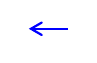
\begin{tikzpicture} \draw[arrows={-angle 60}, white, thick, rotate=180, opacity=1.0] (0,0.00) -- (0.5,0.00); \draw[arrows={-angle 60}, blue, thick, rotate=180] (0,-0.06) -- (0.5,-0.06); \end{tikzpicture}\xspace}
\newcommand{\redline}{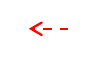
\begin{tikzpicture} \draw[dashed, arrows={-angle 60}, white, thick, rotate=180, opacity=1.0] (0,0.00) -- (0.5,0.00); \draw[dashed, arrows={-angle 60}, red, thick, rotate=180] (0,-0.06) -- (0.5,-0.06); \end{tikzpicture}\xspace}


\usepackage{verbatim}







\icmltitlerunning{Explicit Planning Helps Language Models in Logical Reasoning}

\begin{document}

\twocolumn[
\icmltitle{Explicit Planning Helps Language Models in Logical Reasoning}



\icmlsetsymbol{equal}{*} %

\begin{icmlauthorlist}
\icmlauthor{Hongyu Zhao}{uchi,ttic,equal}
\icmlauthor{Kangrui Wang}{uchi,ttic}
\icmlauthor{Mo Yu}{wechat}
\icmlauthor{Hongyuan Mei}{ttic}
\end{icmlauthorlist}

\icmlaffiliation{uchi}{University of Chicago}
\icmlaffiliation{wechat}{WeChat AI}
\icmlaffiliation{ttic}{Toyota Technological Institute at Chicago}

\icmlcorrespondingauthor{Hongyu Zhao}{hongyuzhao264@gmail.com}
\icmlcorrespondingauthor{Hongyuan Mei}{hongyuan@ttic.edu}

\icmlkeywords{logical reasoning, language model, planning, adversarial}

\vskip 0.3in
]



\printAffiliationsAndNotice{\icmlEqualContribution} %

\begin{abstract}
Language models have been shown to perform remarkably well on a wide range of natural language processing tasks. 
In this paper, we propose a novel system that uses language models to perform multi-step logical reasoning. 
Our system incorporates explicit planning into its inference procedure, thus able to make more informed reasoning decisions at each step by looking ahead into their future effects. 
Moreover, we propose a training strategy that safeguards the planning process from being led astray by spurious features. 
Our full system significantly outperforms other competing methods on multiple standard datasets. 
When using a T5 model as its core component, our system performs competitively compared to GPT-3 despite having only about 1B parameters (i.e., 175 times smaller than GPT-3). 
When using GPT-3.5, it significantly outperforms chain-of-thought prompting on the challenging PrOntoQA dataset. 
We have conducted extensive empirical studies to demonstrate that explicit planning plays a crucial role in the system's performance.
\end{abstract}

\section{Introduction}
\label{sec:introduction}

Logical reasoning is one of the most important and longstanding problems in artificial intelligence~\citep{russel2010}.
A logical reasoning system is able to draw new facts by applying known rules to known facts and determine the truth value of a given hypothesis; see \cref{fig:overview} for an example. 
For decades, research in building reasoning systems has heavily relied on formal logic; %
since the surge of pretrained large language models (LMs), there have been efforts that harness the power of pretrained LMs and directly handle natural language statements to perform multi-step logical reasoning (see \cref{sec:related} for a summary). %
In this paper, we propose the first LM-based logical reasoning system that performs \emph{explicit planning} during inference. 

\paragraph{Why planning?}
Planning is a fundamental property of intelligent behavior: it uses foresight to anticipate future outcomes of each possible decision and informs the process of decision making to achieve desirable end results. %
This concept has influenced the development of various methods in the field of artificial intelligence. 
Minimax-style game playing evaluates each possible move by anticipating replies and counterreplies between the player and the opponent (while assuming that both play optimally)~\citep{russel2010}. 
Model-based reinforcement learning uses environment models to simulate responses to actions and then uses the simulated experiences to help learn value functions (e.g., Dyna, Monte-Carlo tree search)~\citep{sutton2018reinforcement}. 
In natural language processing, planning has been used to help language models generate utterances that satisfy complex constraints~\citep{lu-etal-2022-neurologic}. 

Particularly, planning is important for logic reasoning. 
While determining the true value of a statement, a logical reasoning system usually has to search over the known facts for those which are relevant and perform multiple rounds of deduction to reach the conclusion. 
Planning will help the system focus on the actually useful (known and deduced) facts at early steps, thus reaching the correct conclusion with fewer rounds of deduction. 
Moreover, a planning-based reasoning system tends to be more interpretable, thus more useful in user-centric and safety-critical scenarios. 
For example, at each round of deduction, planning will explicitly show ``what will happen after---and that is also why---I select these known facts and deduce this particular new fact from them'', which is more informative than only saying ``I select these and deduce this.'' 
However, none of the existing LM-based systems use explicit planning during inference. 


\paragraph{Why is it challenging?}
While determining the truth value of a statement, planning examines which reasoning decision (i.e., selection and deduction at each step) is more likely to deduce a fact that definitively proves or disapproves the given statement. 
Ideally, the ``prove or disapprove'' is judged by an oracle such that planning definitely benefits the system by consulting the oracle. 
However, an automated system has to rely on a model to make that judgement (like model-based reinforcement learning), and models are imperfect due to architectural biases and finite training data. 
As a result, it faces the problem of model exploitation: any model mistake may misguide the planning such that it favors a seemingly promising decision over the actually correct one.
For example, the model may incorrectly think a statement proves the hypothesis, just because of a significant lexical overlap, causing the planning to favor a decision that helps deduce that statement and lead to the wrong conclusion. 


\paragraph{Our contributions.}

We first propose a logical reasoning system along with a beam-search-style inference algorithm (\cref{sec:baseline}): the system utilizes pretrained LMs and mimics human-like step-by-step reasoning; its relations with other LM-based systems are discussed in \cref{sec:related}. 
Then we integrate explicit planning into the inference algorithm (\cref{sec:infplan}) and significantly improve the performance of the system. 
We also empirically demonstrate that planning encounters the issue of model exploitation: when the given hypothesis is false, planning may still find out a reasoning path which fools the system to believe that the hypothesis has been proved. % 
Finally, we develop a training strategy that effectively mitigates the issue of model exploitation (\cref{sec:contrastive}). 
Our training strategy is adversarial: 
for each training theory, we synthesize a non-provable hypothesis but call the planning-based inference method to find a highly-scored reasoning path for it; 
then we refine the judging model such that the score it assigns to that path is suppressed; 
at the same time, we force the judging model to preserve its scores on the correct reasoning paths of the provable hypothesises. 
Our experiments show that this strategy further significantly improves the performance of our system. 





\section{Problem Formulation}
\label{sec:problem}
We consider the problem of logical reasoning. 
Given a hypothesis (a.k.a., goal) $\vec{x}_0$ and a theory $\set{T} = \{ \vec{x}_1, \ldots, \vec{x}_N \}$, we are interested in determining the truth value of $\vec{x}_0$, i.e., whether $\vec{x}_0$ can be logically proved by $\set{T}$. 
If the goal $\vec{x}_0$ is provable, we are interested in discovering the reasoning process that proves it. 
Below is an example theory $\set{T}$
\[
    \left\{
    \begin{aligned}
      &\text{``Richard is a King.''}\quad \text{``John is also a King.''}\\
      &\text{``John is greedy.''}\quad \text{``A greedy King is evil.''}
    \end{aligned}
    \right\}
\]
For the goal $\text{``John is evil.''}$, humans can easily verify that it is provable by figuring out the following reasoning path: we can select the two premises about ``John'' and deduce ``John is a greedy King.'' by combining them; we then pick the premise about ``greedy King'' and conclude ``John is evil.'' by combining it with the previous deduction. 
In this paper, we build an automatic system that is able to perform the above human-like logical reasoning.%
\begin{figure}
     \centering
     \begin{center}
        \includegraphics[width=0.9\linewidth]{figures/examples/inference-without-planning.pdf}
        \caption{An example of theory $\set{T}$ and goal $\vec{x}_0$ as well as the logical reasoning process that reaches the goal from the theory.}
        \label{fig:overview}
    \end{center}
\end{figure}



\section{Our Methods}
\label{sec:method}
We propose to build an LM-based logical reasoning system that does explicit planning. 
Conceptually, pretrained LMs are excellent at understanding natural languages as well as fluently generating them.\footnote{We use ``language model'' broadly to include multiple types of language representation models such as encoder-only (BERT, DeBERTa), decoder-only (GPT), and encoder-decoder (T5) models.}
So our system harnesses such abilities to simulate step-by-step reasoning processes that resembles how humans do logical reasoning. 
\cref{fig:overview} illustrates how our system works: %
at each step, 
\begin{itemize}[leftmargin=*,noitemsep,topsep=0pt]
\item it selects a couple of premises from the current theory. E.g., at step-1, it selects ``eagles eat rabbits'' and ``rabbits are animals'' from the original theory of four premises. 
\item it generates a new statement that is logically plausible conditioned on the selected premises, and adds it to the theory whose size then increases by one. E.g., at step-1, it deduces ``eagles eat animals'' which then becomes part ($\vec{x}_5$) of the extended theory. 
\item it scores the new statement by whether it proves the goal. E.g., the score of ``eagles only eat animals'' ($\vec{x}_6$) will be lower than that of ``eagles are carnivores'' ($\vec{x}_7$) since the latter is exactly the same as the goal.
\item it stops if some termination condition is met (e.g., max number of steps reached); otherwise, it starts a new round of selection and deduction. 
\end{itemize}


In the following subsections, we will incrementally build up our system, starting from a base system (\cref{sec:baseline}) 
to how explicit planning is integrated (\crefrange{sec:infplan}{sec:contrastive}).%



\subsection{A Base System}\label{sec:baseline}
The base system consists of three key components: a selection model $p_{\text{sel}}$, a deductioin model $p_{\text{ded}}$, and a verification model $p_{\text{ver}}$.
All these components have pretrained language models at their cores. 
\begin{figure*}
     \centering
     \begin{center}
     \begin{subfigure}[b]{0.45\linewidth}
         \centering
         \includegraphics[width=\linewidth]{figures/structure/selection.pdf}
         \vspace{-16pt}
        \caption{A zoom-in view of the second selection step. The T5 encoder reads some special tokens, the goal $\vec{x}_0$, and the theory $\set{T}$. The decoder computes $p_{\text{sel}}(\vec{x}_n\mid \set{T},\vec{x}_0)$ which is used to evaluate each possible multi-statement selection.}
        \label{fig:sel}
     \end{subfigure}
     \hfill
     \begin{subfigure}[b]{0.45\linewidth}
         \centering
         \includegraphics[width=\linewidth]{figures/structure/deduction.pdf}
         \vspace{-16pt}
        \caption{A zoom-in view of the second deduction step. The T5 encoder reads special tokens and the selection $\vec{s}=\vec{x}_4\ \vec{x}_5$ and generates a deduction autoregressively. It is currently trying to figure out the token after ``only'' and ``eat'' wins.}
        \label{fig:ded}
     \end{subfigure}
    \vspace{-4pt}
    \caption{An illustration of how the selection and deduction models work in the example procedure of \cref{fig:overview}.}
    \label{fig:selded}
    \end{center}
\end{figure*}

\paragraph{Selection model.} The selection model $p_{\text{sel}}$ uses a pretrained encoder-decoder model T5~\citep{raffel2020exploring}. The encoder reads a context string concatenating the goal $\vec{x}_0$ and the premises $\vec{x}_1,\ldots,\vec{x}_N$ of current theory $\set{T}$; the decoder computes the probabilities \mbox{$p_{\text{sel}}(\vec{x}_n\mid \set{T},\vec{x}_0)$} that each premise $\vec{x}_n$ is selected in the attempt to prove the goal $\vec{x}_0$.
It is illustrated in \cref{fig:sel}: 
besides the statements, T5 also reads a few special tokens ($\text{ENC}, \text{SP}_0, \text{SP}_1,\ldots,\text{SP}_N, \text{DEC}$); its decoder gives a hidden state $\vec{h}$, which is involved in computing $p_{\text{sel}}(\vec{x}_n\mid \set{T},\vec{x}_0) \defeq \sigma(\vec{h}^{\top} \vec{w}_{n})$ 
where $\vec{w}_{n}$ is the embedding of $\text{SP}_n$. 
For training and inference efficiency, we keep the pretrained T5 frozen so the only trainable parameters of the selection model $p_{\text{sel}}$---denoted as $\vec{\theta}_{\text{sel}}$---are the embeddings of the special tokens. 

For any multi-premise combination $\vec{s}$ (e.g., $\vec{s}=\vec{x}_2\ \vec{x}_4$), 
the probability $p(\text{statements in }\vec{s}\text{ are selected} \mid \set{T}, \vec{x}_0)$
is\footnote{We treat each $\vec{x}_n$ independently.}
\begin{align*}
    \prod_{n:\vec{x}_n\in\vec{s}} p_{\text{sel}}(\vec{x}_n \mid \set{T}, \vec{x}_0) \prod_{n:\vec{x}_n\notin\vec{s}} (1-p_{\text{sel}}(\vec{x}_n \mid \set{T}, \vec{x}_0))
\end{align*}
Then finding the most probable multi-premise selection is to choose the premises $\vec{x}_n$ that have $p_{\text{sel}}(\vec{x}_n\mid \set{T},\vec{x}_0) > 0.5$.\footnote{For each $\vec{x}_n$, if $p_{\text{sel}} > 0.5$, we will have $p_{\text{sel}} > 1-p_{\text{sel}}$. That is, including it in $\vec{s}$ will increase the probability of $\vec{s}$.}
%

Given a ground-truth multi-premise selection $\vec{s}$ (conditioned on the current theory $\set{T}$ and goal $\vec{x}_0$), one can learn the parameters $\vec{\theta}_{\text{sel}}$ of the selection model by locally maximizing %
\begin{align}
    u = \log p(\text{statements in }\vec{s}\text{ are selected} \mid \set{T}, \vec{x}_0) \label{eqn:sel}
\end{align}
Note that we need a corpus of theories and goals as well as their ground-truth reasoning processes to train the selection model (and the deduction model, as we will show shortly). 
For example, in \cref{fig:overview}, the selection steps (green background) are training examples for $p_{\text{sel}}$:
\begin{itemize}[leftmargin=*,noitemsep,topsep=0pt]
    \item $\set{T}= \{\vec{x}_1, \vec{x}_2, \vec{x}_3, \vec{x}_4\}$ \ \ \ \ \ \ \ \ \ \ \ \ and $\vec{s} = \vec{x}_2 \ \vec{x}_3$
    \item $\set{T}= \{\vec{x}_1, \vec{x}_2, \vec{x}_3, \vec{x}_4, \vec{x}_5\}$ \ \ \ \ \ \ and $\vec{s} = \vec{x}_4 \ \vec{x}_5$
    \item $\set{T}= \{\vec{x}_1, \vec{x}_2, \vec{x}_3, \vec{x}_4, \vec{x}_5, \vec{x}_6\}$ and $\vec{s} = \vec{x}_1 \ \vec{x}_6$
\end{itemize}





\paragraph{Deduction model.}
Given the selection $\vec{s}$, the deduction model $p_{\text{ded}}$ produces a logical deduction $\vec{y}$ by combining the premises in $\vec{s}$. The new statement $\vec{y}$ is added to the theory $\set{T}$ whose size is then increased by one; therefore, for a theory of size $N$, we also denote $\vec{y}$ as $\vec{x}_{N+1}$. 
The deduction model $p_{\text{ded}}$ uses another pretrained T5. As shown in \cref{fig:ded}, its encoder reads an input string concatenating the selected premises along with a few special tokens; its autoregressive decoder produces a deduction one token after another.
Its trainable parameters $\vec{\theta}_{\text{ded}}$ are the embeddings of the special tokens.

For each given pair of $\vec{s}$ and $\vec{y}$, the training objective of learning $\vec{\theta}_{\text{ded}}$ is the log-probability $\log p_{\text{ded}}(\vec{y} \mid \vec{s})$, a typical training objective of similar language generation models. 
In the example of \cref{fig:overview}, the deduction steps (blue background) are training examples for $p_{\text{ded}}$: 
\begin{itemize}[leftmargin=*,noitemsep,topsep=0pt]
    \item $\vec{s} = \vec{x}_2 \ \vec{x}_3$ and new statement $\vec{x}_5$
    \item $\vec{s} = \vec{x}_4 \ \vec{x}_5$ and new statement $\vec{x}_6$
    \item $\vec{s} = \vec{x}_1 \ \vec{x}_6$ and new statement $\vec{x}_7$
\end{itemize}

The selection-deduction mechanism of our system is general: in principle, the selection and deduction models can use any pretrained decoder-only or encoder-decoder model as cores. 
We choose T5---or more precisely, the T5-small instance that has only 60M parameters---because we aim to build a \emph{small} system that works well in practice. As we will see shortly in \cref{sec:experiment}, this small system indeed works well. 

\paragraph{Verification model.}
Ideally, we would like an oracle to tell us whether the goal has been proved at each step. 
A human can do it, but it will be prohibitively expensive to involve a human into this process that is supposed to be automatic and deployed at a large scale. 
Therefore, we use as a substitute a pretrained DeBERTa~\citep{he2021deberta} fine-tuned on the standard MNLI language inference dataset~\citep{mnli}. 
For a statement $\vec{x}_n$ and goal $\vec{x}_0$, the model gives us the probability $p_{\text{ver}}(\vec{x}_0 \mid \vec{x}_n)$ that $\vec{x}_n$ entails $\vec{x}_0$, which we interpret as ``$\vec{x}_n$ proves $\vec{x}_0$''.\footnote{They are not exactly the same, but fairly close.}
Since $p_{\text{ver}}(\vec{x}_0 \mid \vec{x}_n) \in (0,1)$ (softmax probability never reaches $0$ or $1$), the goal $\vec{x}_0$ will never be \emph{definitively} proved and the reasoning process will always reach the maximum number of steps. 
So we define 
\begin{align}
    f(\set{T}, \vec{x}_0)
    \defeq \max_{n=1,\ldots,N} p_{\text{ver}}(\vec{x}_0 \mid \vec{x}_n) \in (0,1) \label{eqn:out}
\end{align}
which can be interpreted as the system's belief that the theory $\set{T}$ can prove the goal $\vec{x}_0$. 
We call it the proof score. 

In the base system, the verification model $p_{\text{ver}}$ is not trained. 

\paragraph{Inference.}
\cref{fig:overview} shows a reasoning path that is obtained by one-best decoding: at each selection or deduction step, the system only takes the choice that is most probable under the model.
However, for a given theory $\set{T}$ and goal $\vec{x}_0$, there may be multiple possible reasoning paths to proving the goal.
Some may be better than the others (e.g., they are shorter) but they may not appear to be promising at the early steps; 
such reasoning paths may be missed by one-best decoding.
Therefore, we propose an improved method that resembles beam search~\citep{jurafsky-2000}.


We maintain a buffer $\set{B}$ of maximum size $B$ which hosts at most $B$ ongoing reasoning paths, which we think are the most promising and will eventually prove the goal. 
Each of ongoing path tracks its proof score $f$ (see \cref{eqn:out}) as well as its log-probability $g$ under our system (defined shortly). 
Both $f$ and $g$ get updated as the path progresses, which we will explain shortly.  
It also tracks its initial theory as well as its previous selections and deductions; the initial theory and the deductions form the current theory. 

As long as we haven't reached the maximum number of steps, we keep expanding each ongoing path in the buffer. 
Each step of expansion includes a selection step followed by a deduction step. 
At the selection step, we do the following: 
\begin{itemize}[leftmargin=*,noitemsep,topsep=0pt]
    \item For each ongoing path, we find its top $B$ most probable selections $(u_1, \vec{s}_1), \ldots, (u_{B}, \vec{s}_{B})$ where $u_b$ is the log-probability (see \cref{eqn:sel}). %
    Each selection expands its ongoing path and updates its $g$ score by $g \gets g + u_b$. 
    \item Now we end up with $|\set{B}| \times B$ extended paths and let the buffer $\set{B}$ only keep at most $B$ paths that are most probable under the system (i.e., they have the highest $g$). 
\end{itemize}
At the deduction step, we follow a similar procedure: 
\begin{itemize}[leftmargin=*,noitemsep,topsep=0pt]
    \item For each ongoing path, we use beam search to draw its top $B$ most probable deductions $(v_{1}, \vec{y}_{1}), \ldots, (v_{B}, \vec{y}_{B})$ conditioned on the most recent selection $\vec{s}$; $v_b$ is the log-probability $p_{\text{ded}}(\vec{y}_b \mid \vec{s})$ under deduction model $p_{\text{ded}}$. 
    Each deduction further expands the ongoing path: it updates the scores by $g \gets g + v_b$ and $f \gets \max\{ f, p_{\text{ver}}(\vec{x}_0\mid \vec{y}_b) \}$.%
    \item Now we end up with $|\set{B}| \times B$ extended paths and only keep at most $B$ of them that have the highest $g$. 
\end{itemize}
In the end, we return the reasoning path with the highest proof score $f$. 
Intuitively, among all the reasoning paths that are probable under the trained selection and deduction models, we would like to pick the one which is most likely to actually prove the goal. 

This method becomes one-best decoding if we set $B=1$. 
%

\paragraph{Relations to formal logic systems.}%
Our base system resembles a rule-based system. 
The inference method is like a combination of the forward and backward chaining algorithms~\citep{russel2010}: at each step, we extend the theory by deducing new facts from the existing facts and rules, which resembles the forward chaining algorithm; each selection step is conditioned on the goal, which resembles the backward chaining algorithm. 
But our proposed method is more flexible. 
Particularly, the forward and backward algorithms can not handle the theories that have non-definite clauses like ``Either John or Richard is evil.''
In principle, our method doesn't have that limitation.%

\paragraph{Technical details.}
More details about the base system are in \cref{app:basesystemdetail,app:inf,app:train}, including the pseudocode for inference (\cref{alg:inf,alg:sel,alg:ded}) and training (\cref{alg:train}).  


\subsection{Improvement-A: Inference with Explicit Planning}\label{sec:infplan}
The inference method in \cref{sec:baseline} lacks \emph{planning}. 
While expanding each ongoing path, the selections and deductions are ranked by their scores $u$ and $v$ that are only conditioned on the previous selections and deductions in the path. 
The method is not concerned with whether the selections and deductions that appear to be promising may actually lead to the \emph{future} steps that are able to prove the goal. 
In this section, we propose an improved inference method that ranks the selections and deductions by explicit planning. %
We call the improved system System-A. 
\begin{figure*}
     \centering
     \begin{center}
     \begin{subfigure}[t]{0.45\linewidth}
         \centering
         \includegraphics[width=\textwidth]{figures/planning/planning-selection.pdf}
         \caption{Planning for selection.}
         \label{fig:plan-sel}
     \end{subfigure}
     \hfill
     \begin{subfigure}[t]{0.45\linewidth}
         \centering
         \includegraphics[width=\textwidth]{figures/planning/planning-deduction.pdf}
         \caption{Planning for deduction.}
         \label{fig:plan-ded}
     \end{subfigure}
    \vspace{-8pt}
    \caption{An illustration of inference with explicit planning at the second selection and deduction step of the full procedure in \cref{fig:overview}.}
    \label{fig:inf-p}
    \end{center}
\end{figure*} 

\paragraph{Planning for selection.}
Suppose that we are now expanding an ongoing path and trying to find out the most promising selections. 
Suppose that there are $K$ different possible multi-premise selections $(u_1, \vec{s}_1), \ldots, (u_K, \vec{s}_K)$ where each $u_k$ is the log-probability of $\vec{s}_k$. 
The naive inference method in \cref{sec:baseline} would have ranked them directly using these log-probabilities. 
However, our improved method will first modify $u_k$ to consider the future steps that $\vec{s}_k$ will lead to and then rank the selections based on the modified $u_k$.%

Precisely, our improved method works as follows. 
It first calls the naive inference method to roll out $D$ steps of future deductions $\tilde{\vec{y}}_{k,1}, \ldots, \tilde{\vec{y}}_{k,D}$ for each possible selection $\vec{s}_k$. For computational efficiency, we set $B=1$ (i.e., one-best search) while rolling out the future steps. 
Then we evaluate how likely each rolled-out deduction may entail the goal, i.e., $p_{\text{ver}}(\vec{x}_0 \mid \tilde{\vec{y}}_{k,d})$, and define $\Delta u_{k} \defeq \max_{d} \log p_{\text{ver}}(\vec{x}_0 \mid \tilde{\vec{y}}_{k,d})$. 
Note that $\Delta u_k$ is just the logarithm of the proof score (see \cref{eqn:out} in \cref{sec:baseline}) defined on the rolled-out future reasoning path. 
Intuitively, a higher $\Delta u_k$ means that this future reasoning path is more likely to prove the goal. 
Then we modify each $u_k$ by $u_k \gets u_k + \alpha \Delta u_k$ where $\alpha$ is a tunable hyperparameter. 
Finally, we find out the top $B$ selections that have the highest modified score $u_k$. 
This improved subroutine is illustrated in \cref{fig:plan-sel}. Its pseudocode is \cref{alg:plan-sel} in \cref{app:plan}. 

\paragraph{Planning for deduction.}
Suppose that we have finished the selection step and are now about to make the deduction step. 
Technically, for each ongoing reasoning path, we need to draw $B$ highest-scored deductions conditioned on the most recent multi-premise selection $\vec{s}$. 
The naive inference method in \cref{sec:baseline} would have used the $B$ deductions given by beam search with size $B$. 
However, our improved method will first over-sample $K > B$ scored deductions $(v_1, \vec{y}_1), \ldots, (v_K, \vec{y}_K)$ by beam search, modify $v_k$ to consider the future steps after choosing $\vec{y}_k$, and then rank the deductions based on the modified $v_k$.%

Precisely, our improved method works as follows. 
It first calls the naive inference method (with $B=1$) to roll out $D$ steps of future deductions $\tilde{\vec{y}}_{k,1}, \ldots, \tilde{\vec{y}}_{k,D}$ for each $\vec{y}_k$.
Then we define $\Delta v_{k} \defeq \max_d \log p_{\text{ver}}(\vec{x}_0 \mid \tilde{\vec{y}}_{k,d})$ (similarly to how we define $\Delta u_k$ at the selection step) and update each $v_k$ by  $v_k \gets v_k + \beta \Delta v_k$ where $\beta$ is a tunable hyperparameter.
Finally, we find out the top $B$ deductions that have the highest {updated} score $v_k$.
This improved subroutine is illustrated in \cref{fig:plan-ded}. Its pseudocode is \cref{alg:plan-ded} in \cref{app:plan}. 

\paragraph{The full method.}
The other parts of our improved inference method are the same as those of the naive method. 
Precisely, the top selections and deductions will expand their ongoing paths and update their proof scores $f$ and log-probabilities $g$ in the same way as in the naive method. 
The buffer then only keeps at most $B$ paths with the highest $g$ like in the naive method. 
However, the improved method will tend to end up with a different set of reasoning paths than the naive method since the scores have been affected by the roll-outs.%

The pseudocode of these two methods is \cref{alg:inf} in \cref{app:inf}: if we set $D=0$, it doesn't roll out future steps and becomes the naive inference method; when $D \geq 1$, it is the improved method that does explicit planning. 


\subsection{Improvement-B: Refined Verification Model}\label{sec:contrastive}
The key limitation of our improved inference method is that explicit planning may exploit the pretrained verification model $p_{\text{ver}}$ such that the final proof score $f(\text{theory}, \text{goal})$ is inflated: this method keeps ongoing paths that have high $p_{\text{ver}}(\text{goal} \mid \text{possible future deductions})$. 
This will result in a high rate of false positive: even when the goal is not provable, explicit planning will still try its best to find out the reasoning paths that have high proof scores; a high proof score will then fool the system itself to believe that this goal is provable. 
This issue is illustrated in our experiments (see \cref{fig:accneg} and related analysis in \cref{sec:binary}). 
In this section, we propose to resolve this issue by refining our verification model. We call the improved system System-B. 

Our method is to tune the verification model $p_{\text{ver}}$ such that $p_{\text{ver}}(\text{goal} \mid \text{deduction})$ is low when the deduction can \emph{not} prove the goal.
Technically, given a theory $\set{T}$ and a \emph{non-provable} goal $\bar{\vec{x}}_0$, we first call our planning-based inference method to find a reasoning path that tries to prove $\bar{\vec{x}}_0$, and then make $p_{\text{ver}}(\bar{\vec{x}}_0 \mid \bar{\vec{y}})$ to be low for each deduction $\bar{\vec{y}}$ in the reasoning path. 
Precisely, we locally minimize $\ell$: 
\begin{align}
    \log p_{\text{ver}}(\bar{\vec{x}}_0 \mid \bar{\vec{y}}) - \log \left( p_{\text{ver}}(\bar{\vec{x}}_0 \mid \bar{\vec{y}}) + p_{\text{ver}}(\vec{x}_0 \mid \vec{y}) \right)
\end{align}
where $\vec{x}_0$ is a provable goal and $\vec{y}$ is a deduction in a reasoning path that actually proves $\vec{x}_0$. 
This objective $\ell$ is a typical contrastive learning objective~\citep{ma2018noise}. 
In our setting, it means: 
if we are given a non-provable goal $\bar{\vec{x}}_0$ paired with a model-proposed reasoning path as well as a provable goal $\vec{x}_0$ paired with a correct reasoning path, 
our verification model $p_{\text{ver}}$ should learn to correctly judge that ``$\bar{\vec{x}}_0$ proved by path of $\bar{\vec{y}}$'' is \emph{less likely} than ``$\vec{x}_0$ proved by path of $\vec{y}$''. This framework is illustrated in \cref{fig:contrast-sample-selection}. %

\begin{figure}
     \centering
     \begin{center}
     \begin{subfigure}[b]{\linewidth}
         \centering
         \includegraphics[width=\textwidth]{figures/others/contrastive_learning.pdf}
         \vspace{-20pt}
         \caption{Illustration of our contrastive learning framework.}
         \label{fig:contrast-sample-selection}
     \end{subfigure}
     
     \begin{subfigure}[b]{\linewidth}
         \centering
         \includegraphics[width=\textwidth]{figures/structure/verification.pdf}
         \vspace{-12pt}
         \caption{The structure of the prompted verification model.}
         \label{fig:verification-structure}
     \end{subfigure}
    \vspace{-24pt}
    \caption{Contrastive refinement of verification model.}
    \label{fig:verification}
    \end{center}
\end{figure} 


Additionally, we augment the loss $\ell$ with %
\begin{subequations}\label{eqn:reg}
\begin{align}
    \Omega 
    =\ 
    &- p^{-}_{\text{ver}}(\vec{x}_0 \mid \vec{y}) \log p_{\text{ver}}(\vec{x}_0 \mid \vec{y}) \\
    &- 
    \left(1-p^{-}_{\text{ver}}(\vec{x}_0 \mid \vec{y})\right) \log \left( 1 - p_{\text{ver}}(\vec{x}_0 \mid \vec{y}) \right)
\end{align}
\end{subequations}
where $p^{-}_{\text{ver}}$ is the pretrained verification model used in \cref{sec:baseline,sec:infplan}. 
It is the KL-divergence (minus $H(p^{-}_{\text{ver}})$, which is a constant wrt.\@ model parameters) between the pretrained and tuned verification models, and minimizing it prevents the tuned model from deviating too much from the pretrained. 
This is desirable since the pretrained model already enjoys a high rate of true positive for provable goals (see \cref{fig:accposi} and relevant analysis in \cref{sec:binary}). 

How do we tune the verification model? 
Like for the selection and deduction models, we use the prompt tuning method~\citep{prompt-tuning}: we augment the input with a few special tokens and the only trainable parameters are the embeddings of those tokens; it is illustrated in \cref{fig:verification-structure}. %

Where do we get $\vec{x}_0$, $\vec{y}$, $\bar{\vec{x}}_0$, and $\bar{\vec{y}}$? %
Recall that we have a training corpus of theories and goals as well as their ground-truth reasoning paths. 
For each pair of theory $\set{T}$ and provable goal $\vec{x}_0$, we could randomly sample a deduction $\vec{y}$ from its ground-truth reasoning path. 
We use the goal of another training example as our non-provable goal $\bar{\vec{x}}_0$, call the planning-based inference method to get a reasoning path, and sample a deduction from the reasoning path as our $\bar{\vec{y}}$. 


\section{Related Work}\label{sec:related}
Reasoning has been a long-standing research topic in the natural language processing community. 
For a long time, the majority of research in this direction has been focused on simple tasks such as single-sentence language inference~\citep{bernardi2002reasoning, zamansky2006natural,maccartney-manning-2009-extended, angeli-etal-2016-combining, hu-etal-2020-monalog, chen-etal-2021-neurallog} and single-step commonsense inference~\citep{rajani-etal-2019-explain,latcinnik2020explaining,shwartz-etal-2020-unsupervised}. %

Recently, there has been an increasing research interest in the more complex problem of multi-step logical reasoning. 
This problem requires multiple steps of non-trivial deduction to determine whether a given natural language hypothesis could be proved by a theory of multiple natural language premises. 
This problem bears the challenges of all the other language inference problems such as language ambiguity and variability. 
In addition, its ``multi-step'' property makes it more difficult: the search space (for a correct reasoning path) is combinatorially large. 
Our paper works in this area. 
\citet{saha-etal-2020-prover}, to the best of our knowledge, is the first to work on this problem. 
They and \citet{tafjord-etal-2021-proofwriter} work on synthesized data of limited language variability.
The LM-based system proposed by~\citet{bostrom2022natural} has an architecture similar to our base system except that their inference is one-best decoding without planning and their deduction model is trained with extra data collected by~\citet{bostrom-etal-2021-flexible}. 
The selection-inference system of~\citet{creswell2022selection} is also similar to our base system but their selection and deduction models are few-shot-prompted GPT-3; we compare with them in \cref{sec:gpt35}. %
\citet{liu-etal-2022-rlet} also use a similar architecture which they train by reinforcement learning. 
Our main contribution is complementary to the related work above: we integrate explicit planning into LM-based reasoning systems and design a training method to mitigate the model exploitation issue that arises in planning. %
Other kinds of approaches to use LMs for reasoning include prompting GPT-3 with spelled-out reasoning procedure~\citep{wei2022chain,talmor2020leap} and distilling GPT-3.5~\citep{fu2023specializing}. 







Another straightforward approach for text-based logical reasoning is to first translate natural language statements into formal logic expressions and then use a formal logic inference engine. 
A lot of efforts have been made in this direction~\cite{weber-etal-2019-nlprolog,levkovskyi2021generating,lu-etal-2022-parsing,betz-richardson-2022-deepa2}, and we also tried it in our experiments. 
However, it turns out to be very challenging to map natural language to formal logic: the translated formal logic expressions often bear subtle issues (e.g., naming variation) such that a formal logic engine won't be able to pattern-match them well.\footnote{
\citet{weber-etal-2019-nlprolog} made this kind of approach to work on WikiHop~\cite{welbl2018constructing} by leveraging dataset-specific properties (e.g., restricted proposition mapping). 
}
\begin{figure*}
     \centering
     \begin{center}
     \begin{subfigure}[b]{0.33\linewidth}
         \centering
         \includegraphics[width=\linewidth]{figures/trained-deberta/roc_fig_test_trained_deberta.pdf}
         \vspace{-16pt}
        \caption{ROC curves.}
        \label{fig:roc}
     \end{subfigure}
     \hfill
     \begin{subfigure}[b]{0.33\linewidth}
         \centering
         \includegraphics[width=\linewidth]{figures/trained-deberta/true_fig_test_trained_deberta.pdf}
         \vspace{-16pt}
        \caption{Accuracy curves on positive examples.}
        \label{fig:accposi}
     \end{subfigure}
     \hfill
     \begin{subfigure}[b]{0.33\linewidth}
         \centering
         \includegraphics[width=\linewidth]{figures/trained-deberta/false_fig_test_trained_deberta.pdf}
         \vspace{-16pt}
        \caption{Accuracy curves on negative examples.}
        \label{fig:accneg}
     \end{subfigure}

    \vspace{-8pt}
    \caption{
    Test results on Entailment Bank Version-I.
    For each curve in the figures, we show its 95\% bootstrap confidence interval. 
    }
    \label{fig:expcurves}
    \end{center}
\end{figure*}
\begin{table*}[t]
\begin{center}
\begin{small}
\begin{sc}
\begin{tabular}{lcccc}
\toprule
Method & AUROC & $\text{AUACC}_{\text{pos}}$ & $\text{AUACC}_{\text{neg}}$ & F1  \\
\midrule
Baseline-T5 & 0.67 (0.63, 0.71) & 0.53 (0.49, 0.57) & 0.75 (0.72, 0.78) & 0.62 (0.59, 0.64) \\
Base System & 0.56 (0.51, 0.60) & 0.42 (0.38, 0.47) & 0.78 (0.76, 0.81) & 0.67 (0.67, 0.67)\\
System A    & 0.87 (0.84, 0.89) & 0.86 (0.84, 0.89) & 0.54 (0.50, 0.57) & 0.82 (0.80, 0.84)\\
System B    & \textbf{0.94} (0.92, 0.95) & \textbf{0.87} (0.84, 0.89) & \textbf{0.82} (0.79, 0.85) & \textbf{0.89} (0.87, 0.91)\\
GPT-3 (0-shot) & - & - & - & \textbf{0.89}\\
\bottomrule
\end{tabular}
\end{sc}
\end{small}
\caption{Test results with 95\% bootstrap confidence intervals on Entailment Bank Version-I. }
\label{tab:mainresultent}
\end{center}
\vskip -0.1in
\end{table*}


Another research area related to multi-step logical reasoning is to reason over graph-structured data. 
A popular kind of graph is knowledge graphs, i.e., relational graphs over symbolic tuples~\cite{lao2010relational,wang2013programming,neelakantan2015compositional,cohen2017tensorlog,xiong2017deeppath,chen2018variational,das2017go}. 
Another kind of graph is built by linking texts via lexical overlap or hyperlink connections~\cite{welbl2018constructing,yang-etal-2018-hotpotqa,khot2020qasc,khot-etal-2021-text}.
In this area, people are interested in answering natural language questions by searching over a graph, which typically requires multi-step navigation through the graph. 
However, such tasks are not good testbeds for deductive reasoning that we work on in this paper, since optimizing the performance on these datasets is not necessarily aligned to improving the models' fundamental reasoning abilities~\cite{chen-durrett-2019-understanding,min-etal-2019-compositional}. 
For example, shortcuts often exist such that one may correctly answer a question by answering some of the subquestions rather than composing the answers to the subquestions. 
Additionally, models trained on such tasks can not directly apply to our setting since they rely on pre-defined symbolic and relational structures. 


















\section{Experiments}
\label{sec:experiment}

We implemented our methods with PyTorch~\citep{pytorch} and Transformers~\citep{huggingface}. Our code can be found at {\small\url{https://github.com/cindermond/explicit-planning-for-reasoning}}.% 
\begin{figure*}
     \centering
     \begin{center}
     \begin{subfigure}[b]{0.33\linewidth}
         \centering
         \includegraphics[width=\linewidth]{figures/low-data/roc_fig_test_657.pdf}
         \vspace{-16pt}
        \caption{ROC curves.}
        \label{fig:roc0.5}
     \end{subfigure}
     \hfill
     \begin{subfigure}[b]{0.33\linewidth}
         \centering
         \includegraphics[width=\linewidth]{figures/low-data/true_fig_test_657.pdf}
         \vspace{-16pt}
        \caption{Accuracy curves on positive examples.}
        \label{fig:accposi0.5}
     \end{subfigure}
     \hfill
     \begin{subfigure}[b]{0.33\linewidth}
         \centering
         \includegraphics[width=\linewidth]{figures/low-data/false_fig_test_657.pdf}
         \vspace{-16pt}
        \caption{Accuracy curves on negative examples.}
        \label{fig:accneg0.5}
     \end{subfigure}

    \vspace{-8pt}
    \caption{Test results with 95\% bootstrap confidence intervals on Entailment Bank Version-I under 50\% training data.}
    \label{fig:expcurves0.5}
    \end{center}
\end{figure*}
\begin{figure*}
     \centering
     \begin{center}
     \begin{subfigure}[b]{0.33\linewidth}
         \centering
         \includegraphics[width=\linewidth]{figures/task2/roc_fig_test_task2.pdf}
         \vspace{-16pt}
        \caption{ROC curves.}
        \label{fig:roctask2}
     \end{subfigure}
     \hfill
     \begin{subfigure}[b]{0.33\linewidth}
         \centering
         \includegraphics[width=\linewidth]{figures/task2/true_fig_test_task2.pdf}
         \vspace{-16pt}
        \caption{Accuracy curves on positive examples.}
        \label{fig:accpositask2}
     \end{subfigure}
     \hfill
     \begin{subfigure}[b]{0.33\linewidth}
         \centering
         \includegraphics[width=\linewidth]{figures/task2/false_fig_test_task2.pdf}
         \vspace{-16pt}
        \caption{Accuracy curves on negative examples.}
        \label{fig:accnegtask2}
     \end{subfigure}

    \vspace{-8pt}
    \caption{Test results with 95\% bootstrap confidence intervals on Entailment Bank Version-II.}
    \label{fig:expcurvestask2}
    \end{center}
\end{figure*}

We have carried out a diverse set of experiments to demonstrated the effectiveness of our proposed methods. 
In \cref{sec:ebsetup,sec:qasc}, we will discuss the experiments where we use small T5 models as the core selection and deduction modules in our framework. 
In \cref{sec:gpt35}, we will discuss the experiments where we use GPT-3.5-turbo as the selection and deduction models. 

\subsection{EntailmentBank Experiments}\label{sec:ebsetup}

We first trained and evaluated our methods on the standard benchmark Entailment Bank~\citep{dalvi-etal-2021-explaining} dataset. 
It is a corpus of human-annotated (theory, provable goal, reasoning path) tuples, including the example in \cref{fig:overview}.% 
This dataset has two versions: in Version-I, for each pair of theory and goal, all the premises have to be used to prove the goal; in Version-II, each theory includes a few distractors that are not useful for proving the goal. 
We trained the models on Version-I training data, but evaluated them on both Version-I and Version-II test data. 

Experiment details can be found in \cref{app:expdetail}, including data statistics (\cref{tab:entailmentbankstats}) and training details (e.g., hyperparameter tuning in \cref{app:hyperpara}).%
%

\paragraph{Evaluation-I: binary classification.}\label{sec:binary}
We evaluated the abilities of the systems to classify provable and non-provable goals. 
For this purpose, we gave a non-provable goal to each dev and test theory by selecting it from other (theory, goal, reasoning path) samples. 
The selection is adversarial: we tuned a pretrained T5 model to generate a provable goal given a theory; for each theory $\set{T}$, we looped over all the goals in the dataset that are guaranteed to be not provable under $\set{T}$, and chose the one that the T5 thinks is the most probable given $\set{T}$ (see details in \cref{app:expdetail}). 


For each given theory $\set{T}$ and goal $\vec{x}_0$, we let the system generate a reasoning path that tries to prove the goal, and obtain the proof score $f(\set{T}, \vec{x}_0)$ of the path. 
Given a threshold $\tau \in (0,1)$, we say ``$\vec{x}_0$ is provable'' if $f(\set{T}, \vec{x}_0) \geq \tau$ and ``$\vec{x}_0$ is not provable'' otherwise. 
For a systematic investigation, we varied $\tau$ and plot a receiver operating characteristic (ROC) curve for each system; the larger the area under ROC curve (AUROC) is, the better the system is. 


The ROC curves are shown in \cref{fig:roc}. 
As we can see, our System-A and System-B substantially and significantly outperform the base system and a T5 model (trained on generating goals given theories), and System-B further significantly outperforms System-A. 
Surprisingly, our base system underperforms the T5 model even though it has learned to spell out its reasoning steps which we expect to help the classification. 


\cref{fig:accposi} and \cref{fig:accneg} show the results broken down into the accuracies on the provable goals and non-provable goals, respectively. 
On provable goals, the accuracy is the number of true positive divided by the total number of test cases; on non-provable goals, the accuracy is the number of true negative divided by the total number of test cases. 
As we can see, System-A works very well on the provable goals, but performs poorly on the non-provable goals. 
That is because System-A exploits the verification model by explicit planning: as we have discussed in \cref{sec:contrastive}, the proof scores given by System-A tend to be high, thus yielding a high rate of false positive. 
System-B works well on both provable and non-provable goals: the refined verification model $p_{\text{ver}}$ successfully avoided being exploited by planning. 

Actual values of the areas under curves are shown in \cref{tab:mainresultent}: $\text{AUACC}_{\text{pos}}$ and $\text{AUACC}_{\text{neg}}$ correspond to the curves in \cref{fig:accposi} and \cref{fig:accneg}, respectively.
The F1 numbers were computed as follows: we chose an optimal threshold $\tau$ by maximizing the F1 score on the development set, and then computed F1 on the test set according to the chosen $\tau$. 
On this metric, we also compared with 0-shot GPT-3-davinci and our System-B performs as well as this strong model. 


\paragraph{Analysis-I: robustness to size of training data.}
We trained the models with (randomly sampled) 50\% of the training data, and re-evaluated them on the same test set. 
The results are shown in \cref{fig:expcurves0.5}: these figures look similar to \cref{fig:expcurves} and our System-B still performs the best.



\paragraph{Analysis-II: About the regularization in \cref{eqn:reg}.} 
We compared the system B with and without the regularization term $\Omega$. %
Without using the regularization, System-B performs worse than System-A. 
Additionally, we evaluated the tuned verification models on the MNLI dataset (on which the model was fine-tuned), and found that: the model tuned without the regularization can only achieve 62.0\% accuracy on the MNLI matched development set; the model tuned with the regularization can achieve 91.4\% accuracy, almost as good as it originally was (91.7\%).
It means that the regularization helps the verification model preserve its ability to judge the entailment relationship.

\paragraph{Analysis-III: Robustness to distractors.} 
We investigated the robustness of the systems to distractors by evaluating them on Version-II test data. 
Note that they were only trained on Version-I training data. 
The results are shown in \cref{fig:expcurvestask2}: all the systems perform worse than they did on Version-I test data, but the performance drop of our systems is much smaller than that of the T5 model. 
It means that our systems are more robust to the distractors in the theories. 
That is perhaps because our systems explicitly spell out their reasoning steps and explicit planning can help the systems (A and B) focus on the premises that are actually relevant to the goal at each selection step.  
We believe that training the models on Version-II training data (or using denoising methods) will further improve the performance.

\paragraph{Analysis-IV: Formal logic approach.}
In \cref{sec:introduction}, we mentioned that the classical approach of logical reasoning is to use formal logic systems. 
In this project, we also evaluated the performance of a first-order-logic (FOL) system. 
Because the Entailment Bank dataset does not have human-annotated FOL translations for the natural language statements, we translated all the statements into FOL expressions using a T5 model trained on the corpus of (natural language, FOL) pairs collected by~\citet{levkovskyi2021generating}, and then used a FOL engine to perform reasoning. 
This approach failed because the FOL translations are mostly of very poor quality. 
Details about this experiment can be found in \cref{app:fol}. 

\paragraph{Analysis-V: About mode size and denoising.}
To examine the effect of model size, we reran the main experiments with T5-small replaced by T5-base which has 220M parameters. 
It turns out that using a larger model achieved a consistently stronger performance and our planning-based systems still significantly outperform the base system. 

We also experimented with denoising training of the selection and deduction models. 
Precisely, every time we used a training example, we randomly permuted the input statements.
The denoising-trained models lead to a better generalization to the evaluation settings with distractors. 
We also found that training with distractors (i.e., using Verstion-II training data) significantly improved the results. 

\cref{tab:sizedenoise} and \cref{tab:sizedenoise2} of \cref{app:ablation} display the results for this set of analysis. 

\paragraph{Evaluation-II: Multiple-Choice Question Answering.}\label{sec:mcqat5}
We further evaluated the systems in a multiple-choice question answering (QA) setting. 
Particularly, given a theory $\set{T}$ in Entailment Bank, each system is asked to select the provable goal from four choices $\{\vec{x}_0^{(1)}, \vec{x}_0^{(2)}, \vec{x}_0^{(3)}, \vec{x}_0^{(4)} \}$: one of them is the ground-truth provable goal while the others are negative choices selected by a tuned T5 (like how we created the binary classification task in \cref{sec:binary}). 
\begin{table}[t]
\begin{center}
\begin{small}
\begin{sc}
\begin{tabular}{lcc}
\toprule
Method & Version-I & Version-II \\
\midrule
Baseline-T5 & 0.60 (0.55, 0.65) & 0.20 (0.16, 0.24) \\
Base System & 0.46 (0.41, 0.52) & 0.29 (0.25, 0.34)\\
System A    & 0.80 (0.76, 0.84) & 0.44 (0.39, 0.49)\\
System B    & \textbf{0.88} (0.85, 0.92) & \textbf{0.63} (0.58, 0.68)\\
\midrule
GPT-3 (0-shot) & 0.72  & 0.20\\
GPT-3 (5-shot) & 0.97  & 0.96\\
GPT-3 (COT) & \textbf{0.98} & \textbf{0.98}\\
\bottomrule
\end{tabular}
\end{sc}
\end{small}
\caption{Test accuracy with 95\% bootstrap confidence intervals in multiple-choice setting. A random guess give 25\% accuracy.}
\label{tab:mainresultqa}
\end{center}
\vskip -0.1in
\end{table}


We took the systems trained in \cref{sec:binary} (i.e., no further task-specific tuning) and evaluated them on the Version-I and Version-II of this multiple-choice task: in the Version-II setting, each theory has a few distractors, so it is more challenging than Version-I. 
For each theory, a system tries to prove each choice $\vec{x}_0^{(c)}$, ranks the four choices by their proof scores $f(\set{T}, \vec{x}_0^{(c)})$, and then chooses the one with the highest score. 
The systems were evaluated by accuracy. 
As shown in \cref{tab:mainresultqa}, the systems behave similarly as they do on the binary classification: in both Version-I and Version-II settings, System-A and System-B perform significantly better than the baselines, and System-B significantly outperforms System-A. 

We also evaluated GPT-3-davinci with 0-shot, 5-shot, and chain-of-thought (COT) prompting~\citep{gpt3,wei2022chain}.
For COT, we included the ground-truth reasoning paths of the correct choices in the prompts; examples can be found in \cref{app:examplegpt3}.
Our full system outperforms 0-shot GPT-3, but underperforms 5-shot and COT GPT-3. 
Interestingly, 0-shot GPT-3 works worse than random guess when theories have distractors, which also indicates the difficulty of this problem. 
















\begin{table*}[h]
\centering
\begin{minipage}{0.32\textwidth}
\centering
\begin{small}
\begin{sc}
\begin{tabular}{lc}
\toprule
Method & Acc \\
\midrule
Base System & 0.68 (0.65, 0.71) \\
System A    & 0.84 (0.82, 0.87) \\
System B    & \textbf{0.85} (0.83, 0.87) \\
\bottomrule
\end{tabular}
\end{sc}
\end{small}
\begin{minipage}[t][1cm][t]{\textwidth}
\caption{Dev accuracy with 95\% bootstrap confidence intervals  on QASC. A random guess give 12.5\% accuracy.}
\label{tab:qasc}
\end{minipage}
\end{minipage}
\hfill
\begin{minipage}{0.65\textwidth}
\centering
\begin{small}
\begin{sc}
\begin{tabular}{lccc}
\toprule
Method & Depth=1 & Depth=3 & Depth=5 \\
\midrule
COT & 0.71 (0.62, 0.80)&\textbf{0.57} (0.47, 0.67)&0.52 (0.42, 0.62)\\
SI & 0.88 (0.81, 0.94) &0.51 (0.41, 0.61)&0.45 (0.35, 0.55)\\
System A &\textbf{0.90} (0.84, 0.95) &0.55 (0.45, 0.65) &\textbf{0.55} (0.45, 0.65)\\
\bottomrule
\end{tabular}
\end{sc}
\end{small}
\begin{minipage}[t][1cm][t]{\textwidth}
\caption{Accuracy with 95\% bootstrap confidence intervals on PrOntoQA with GPT-3.5 as the selection and deduction models. The ``depth'' means the length of the ground-truth reasoning paths. Each depth contains 5 training examples and 100 test examples. }
\label{tab:prontoqa}
\end{minipage}
\end{minipage}
\end{table*}

\subsection{QASC Experiments}\label{sec:qasc}
We also trained and evaluated the systems on the QASC dataset~\citep{khot2020qasc}, a multiple-choice question answering dataset where each question has eight candidate answers. 
Each training QA pair has two premises and a deduction, which can be used to train our deduction model. 
Each development QA pair has two premises so the reasoning system only needs to do a step of deduction but no selection. 
Test QA pairs have no premises given and one has to search through a pool of millions of statements to find the relevant premises, which is not the focus of this paper. 
So we only evaluated the systems on the development set. 
The results are in \cref{tab:qasc}. 
Although this data only requires one step of reasoning, the planning-based systems still significantly outperform the base system, meaning that explicit planning is indeed helpful for LM-based reasoning. 



\subsection{GPT-3.5 as Selection and Deduction Models}\label{sec:gpt35}
So far we have only presented the results of using small language models in our framework. 
In this section, we discuss our experiments in which we use GPT-3.5-turbo as our selection and deduction models. 
GPT-3.5 is the current largest and state-of-the-art language model that we have access to. 
Our system still works step by step as in \cref{fig:overview}: at each step, we instruct GPT-3.5 to perform selection and deduction by few-shot prompting. 
This is similar to the selection-inference framework proposed by~\citet{creswell2022selection} except that we request GPT-3.5 to propose multiple possible selections and deductions at each step. 
This design allows us to perform explicit planning for each possible selection and deduction and then choose the best option based on planning. 
In this set of experiments, our final verification is also performed by a few-shot-prompted GPT-3.5: it reads the extended theory and judges whether the given goal is proved. 

We evaluated the GPT-3.5-based system on the ``fictional'' version of the PrOntoQA dataset~\citep{SaparovHe22}. 
It is challenging since its logical statements are about fictional characters (e.g., wumpus) so a large language model like GPT-3.5 can not bypass the reasoning and draw correct conclusions by commonsense or memorization. 
It is a binary classification task like EntailmentBank (\cref{sec:binary}), but the key difference is that its non-provable goals are often definitively disapprovable. 
So we would like the explicit planning to favor not only the future steps that have large proof scores but also those of large \emph{contradiction} scores. 
Therefore, we replace the proof score $f$ in the planning procedure by the $g$ defined below 
\begin{align}
    g(\set{T}, \vec{x}_0)
    \defeq \max_{n} \max(p_{\text{ver}}(\vec{x}_0 \mid \vec{x}_n), p_{\text{con}}({\vec{x}}_0 \mid \vec{x}_n))
    \label{eqn:proofscorenew}
\end{align}
where $p_{\text{con}}({\vec{x}}_0 \mid \vec{x}_n)$ is the probability of ``$\vec{x}_n$ contradicts $\vec{x}_0$'' given by the pretrained DeBERTa. 
Please see \cref{app:ablation} for how much this modification helps. 


The results are shown in \cref{tab:prontoqa}. 
In all cases, our system outperforms the selection-inference (SI) method, meaning that explicit planning is consistently helpful. 
In most cases, our planning-based system performs better than the strong chain-of-thought (COT) prompting. %
We also experimented with the DeBERTa model tuned on the EntailmentBank training data (\cref{sec:contrastive,sec:binary}) and found that it couldn't improve the performance on PrOntoQA. 
More results can be found in \cref{tab:prontoqaablabtionstudy} of \cref{app:ablation}. 

\section{Conclusion and Future Work}
\label{sec:conclusion}
In this paper, we presented an LM-based logical reasoning system that integrates explicit planning into the inference method. 
Additionally, we proposed a method that learns to prevent the explicit planning from being misguided. 
In our experiments, our planning-based systems outperform strong baseline methods including the selection-inference method and chain-of-thought prompting. 
This has inspired us to explore several exciting avenues for further improvements. 

The first is to jointly refine the selection, deduction, and verification models. 
In this paper, we have already shown that adversarially refining the verification model will significantly improve the performance. 
So a natural next step is to also adversarially refine the selection and deduction models in response to the updated verification model. 
Allowing components of a system to adversarially refine one another has been shown useful in the natural language processing community~\cite{yu2019rethinking}.


The second is to develop \emph{implicit} planning methods to improve inference efficiency. 
In reinforcement learning, explicit planning is often only used to help learn a value function during training; during inference, calling a value function is like planning implicitly but faster than explicit planning. 
This kind of methods can apply to our setting. 

Another direction is to leverage unlabeled data, i.e., data without human-annotated reasoning paths.
Such data is less expensive to collect. %
An LM-based logical reasoning system may be able to benefit from (the indirect training signals of) such data by self-supervised learning. 

\section*{Acknowledgements}
This work was supported by a research gift to the last author by Adobe Research. 
We thank our colleagues at Toyota Technological Institute at Chicago and University of Chicago for helpful discussion. 



%


%

%


\bibliography{hongyu_nlp}
\bibliographystyle{icml2020_url}


\clearpage
\newpage
\appendix


\section{Method Details}\label{app:methoddetail}

\subsection{Base System Details}\label{app:basesystemdetail}

\paragraph{Why prompt learning?}
We use pretrained Text-To-Text Transfer Transformer (T5) language models~\citep{raffel2020exploring} for both modules.
We use prompt-learning because we do not want to distort the pretrained weights too much. 
It is well known that pretrained language models have already captured substantial amounts of commonsense knowledge such as hypernymy (A is a type of B) and meronymy (A is part of B)~\citep{richardson-sabharwal-2020-qa}; we would like to keep such knowledge to benefit our settings. 

\subsection{Reasoning Process Details}\label{app:inf}

\cref{alg:inf} gives a detailed explanation for how our inference method works. When $D = 0$, it is the naive method. When $D \geq 1$, it is the inference with explicit planning. 
During selection, we constrain the model to only select two premises for a more controllable behavior. 
When we compute the proof score we only consider the newly generated deductions for convenience. Its effect to results is negligible since later deductions tend to more directly prove the goal. 

\cref{alg:sel} is designed to select a set of statements from the current theory $\set{T}$, with the goal of inferring $\vec{x}_0$. We fix the size of the selection set to 2 in our experiments, but in principle this restriction can be removed.

\cref{alg:ded} applies the standard beam search method to the generation of new deduction. $B_{\text{ded}}$ deductions with top scores are selected.


\begin{algorithm}
\caption{Reasoning (Inference) with Our System}\label{alg:inf}
\begin{algorithmic}[1]
    \HYPER maximum number of inference steps $M$;\newline
    depth of planning $D$ ($D=0$ means ``no planning'');\newline
    inference beam size $B_{\text{inf}}$ %
    \INPUT theory $\set{T}=\{\vec{x}_1,\vec{x}_2,\ldots,\vec{x}_{N}\}$ and goal $\vec{x}_0$;\newline
    selection model $p_{\text{sel}}$, deduction model $p_{\text{ded}}$;\newline 
    verification model $p_{\text{ver}}$
    \OUTPUT reasoning path $\set{R}$ with proof score $f$%
  \Procedure{Inference}{$\set{T}, \vec{x}_0, p_{\text{sel}}, p_{\text{ded}}, p_{\text{ver}}$}
    \LineComment{has access to $M$, $B_{\text{inf}}$, $D$}
    \State $\set{B} \gets \text{PriorityQueue}(B_{\text{inf}})$
    \LineComment{max size is $B_{\text{inf}}$ ; priority is first element of tuple}
    \State $\set{B}.\text{add}((0, \emptyset, \set{T}, -\infty))$ 
    \LineComment{init with empty path and current theory}
    \For{$m = 1$ {\bfseries to} $M$}
        \LineComment{do inference at each step}
        \LineComment{selection at step $m$}
        \State $\set{B}_{\text{old}} \gets \set{B}$; 
        $\set{B} \gets \text{PriorityQueue}(B_{\text{inf}})$
        \For {$g_b, \set{R}_b,\set{T}_b, f_b$ {\bfseries in} $\set{B}_{\text{old}}$} %
            \LineComment{$g$ is log-prob of path and $f$ is its proof score}
            \State $\set{S}_b \gets \textsc{Select}(\set{T}_b, \vec{x}_0, p_{\text{sel}})$
            \If {$D > 0$}  
                \LineComment{rerank selections based on $D$ steps of roll-outs}
                \State $\set{S}_b \gets \textsc{PlanSel}(\set{T}_{b},\vec{x}_0,\set{S}_b, p_{\text{sel}}, p_{\text{ded}}, p_{\text{ver}})$
            \EndIf
            \For{$u_k, \vec{s}_k$ in $\set{S}_b$}
                \LineComment{add expanded reasoning path into priority queue}
                \LineComment{priority score changes by $u_k$}
                \State $\set{B}.\text{add}((g_b+u_k, \set{R}_{b}+\{\vec{s}_k\}, \set{T}_b, f_b))$
                \LineComment{if $|\set{B}| > B_{\text{inf}}$, auto-delete lowest-priority element}
            \EndFor
        \EndFor
        \LineComment{deduction at step $m$}
        \State $\set{B}_{\text{old}} \gets \set{B}$; 
        $\set{B} \gets \text{PriorityQueue}(B_{\text{inf}})$
        \For {$g_b, \set{R}_b,\set{T}_b, f_b$ {\bfseries in} $\set{B}_{\text{old}}$} 
            \State $\vec{s}_b \gets$ the most recent selection in $\set{R}_b$
            \State $\set{Y}_b \gets \textsc{Deduce}(\vec{s}_b, p_{\text{ded}})$ 
            \If {$D > 0$}  
                \LineComment{rerank deductions based on $D$ steps of roll-outs}
                \State $\set{Y}_b \gets \textsc{PlanDed}(\set{T}_{b}, \vec{x}_0, \set{Y}_b, p_{\text{sel}}, p_{\text{ded}}, p_{\text{ver}})$
            \EndIf
            \For{$v_k, \vec{y}_k$ in $\set{Y}_b$}
                \State $\set{B}.\text{add}((g_b + v_k, \set{R}_{b}+\{\vec{y}_k\}, \set{T}_b + \{\vec{y}_k\}, f_b))$
            \EndFor
        \EndFor       
        \For {$g_b,\set{R}_b,\set{T}_b,f_b$ {\bfseries in} $\set{B}$ }
            \State $\vec{y}_b \gets$ the most recent deduction in $\set{R}_b$
            \LineComment{if $\vec{y}_b$ entails $\vec{x}_0$ better than any prev deduction}
            \LineComment{update proof score of path $\set{R}_b$}
            \IfThen{$p_{\text{ver}}(\vec{x}_0\mid \vec{y}_b) > f_b$}{$f_b \gets p_{\text{ver}}(\vec{x}_0\mid \vec{y}_b)$}
        \EndFor
    \EndFor
    \LineComment{choose reasoning path with highest proof score}
    \State $b_{\text{max}} \gets \argmax_bf_b$
    \State \textbf{return} $\set{R}_{b_{\text{max}}}, f_{b_{\text{max}}}$
  \EndProcedure
\end{algorithmic}
\end{algorithm}



\begin{algorithm}
\caption{Selection Subroutine}\label{alg:sel}
\begin{algorithmic}[1]
    \HYPER{selection beam size $B_{\text{sel}}$}
    \INPUT current theory $\set{T} = \{\vec{x}_1,\ldots,\vec{x}_{N+m}\}$ and goal $\vec{x}_0$;\newline
        prompted encoder-decoder language model $p_{\text{sel}}$%
        \OUTPUT selections with their scores $\{(u_k,\vec{s}_k)\}$
  \Procedure{Select}{$\set{T}, \vec{x}_0, p_{\text{sel}}$}
      \LineComment{has access to $B_{\text{sel}}$}
      \LineComment{construct context by concatenating hypothesis and theory}
  \State $\vec{c} = \text{SP}_0 + \vec{x}_0 + \text{SP}_1 + \vec{x}_1 + \ldots + \text{SP}_{N+m} + \vec{x}_{N+m}$
   \For{$i = 1$ {\bfseries to} $N+m$}  
        \LineComment{compute probability that each statement is selected}
        \State $p_i \gets p_{\text{sel}}(\text{SP}_i|\vec{c})$
   \EndFor
   
  \State $\set{S} \gets \text{PriorityQueue}(B_{\text{sel}})$
  \LineComment{max size is $B_{\text{sel}}$; priority is first element of tuple}
  \For{$i = 1$ {\bfseries to} $N+m$}
    \For{$j = i+1$ {\bfseries to} $N+m$}
        \State $\vec{s}_{k} \gets \vec{x}_{i} + \vec{x}_{j}$
        \State $u_{k} \gets \log p_i + \log p_j + \sum_{\ell \neq i,\ell\neq j}\log(1-p_{\ell})$
        \State $\set{S}.\text{add}((u_k, \vec{s}_k))$
        \LineComment{if $\set{B}$ is larger than $B_{\text{sel}}$, element with lowest priority}
        \LineComment{will be automatically deleted}
    \EndFor
  \EndFor
  \State \textbf{return} $\set{S}$
  \EndProcedure
\Procedure{OneBestSelect}{$\set{T}, \vec{x}_0, p_{\text{sel}}$} 
    \LineComment{only keeps selection with highest score}
  \State $\set{S} \gets \textsc{Select}(\set{T},\vec{x}_0, p_{\text{sel}})$
  \State $(u, \vec{s}) \gets$ top element in priority queue $\set{S}$
  \State \textbf{return} $\vec{s}$
  \EndProcedure
\end{algorithmic}
\end{algorithm}



\begin{algorithm}
\caption{Deduction Subroutine}\label{alg:ded}
\begin{algorithmic}[1]
        \HYPER deduction beam size $B_{\text{ded}}$
	\INPUT current selection $\vec{s}$ of statements;\newline 
                prompted encoder-decoder language model $p_{\text{ded}}$ 
        \OUTPUT deductions with their scores $\{(v_k, \vec{y}_k)\}$
  \Procedure{Deduce}{$\vec{s}$, $p_{\text{ded}}$}
      \LineComment{has access to $B_{\text{ded}}$}
      \LineComment{has access to a standard beam search implementation} 
    \State $\set{Y} \gets \textsc{BeamSearch}(p_{\text{ded}},B_{\text{ded}},\vec{s})$
    \LineComment{assume \textsc{BeamSearch} gives a list of tuples $\{(v_k, \vec{y}_k)\}$}
    \LineComment{sorted in descending order of $v_k$, each $\vec{y}_k$ is a text string}
    \State \textbf{return} $\set{Y}$
  \EndProcedure
    \Procedure{OneBestDeduce}{$\vec{s}$, $p_{\text{ded}}$}  \LineComment{only keeps deduction with highest score}
    \State $\set{Y} \gets \textsc{Deduce}(\vec{s}, p_{\text{ded}})$
    \State $(v, \vec{y}) \gets$ element in $\set{Y}$ with highest $v$
    \State \textbf{return} $\vec{y}$
  \EndProcedure
\end{algorithmic}
\end{algorithm}






\subsection{Details of Training Methods}\label{app:train}
\cref{alg:train} elaborates how the system is trained. 

\begin{algorithm}
\caption{Training}\label{alg:train}
\begin{algorithmic}[1]
    \INPUT 
    theory $\set{T}=\{\vec{x}_1, \ldots, \vec{x}_{N}\}$ and goal $\vec{x}_0$;\newline
    reasoning path $\set{R}$; verification model $p_{\text{ver}}$\newline 
    selection model $p_{\text{sel}}$, deduction model $p_{\text{ded}}$
    \OUTPUT updated models $p_{\text{sel}}$ and $p_{\text{ded}}$
  \Procedure{Train}{$\set{R}, \set{T}, \vec{x}_0, p_{\text{sel}}, p_{\text{ded}}, p_{\text{ver}}$}
    \LineComment{training procedure for selection and deduction models}
    \State $\tilde{\set{T}} \gets \set{T}$ \Comment{init extended theory that will include deduction}
    \For{$m = 1$ {\bfseries to} $|\set{R}|/2$} 
        \LineComment{loop over each step of selection and deduction}
        \State $\vec{s}_m\gets$ $m$\th selection \Comment{i.e., $(2m-1)$\th element in $\set{R}$}
        \State $\vec{y}_m\gets$ $m$\th deduction \Comment{i.e., $(2m)$\th element in $\set{R}$}
        \LineComment{train selection model}
        \State $\ell \gets \textsc{LossSel}(\tilde{\set{T}}, \vec{s}_m, p_{\text{sel}})$
        \State compute $\nabla \ell$ wrt.\@ trainable parameters $\vec{\theta}_{\text{sel}}$ of $p_{\text{sel}}$
        \State update $\vec{\theta}_{\text{sel}}$ with chosen optimization method
        
        \LineComment{train deduction model}
        \State $\ell \gets \textsc{LossDed}(\vec{s}_m, \vec{y}_m,p_{\text{ded}})$
        \State compute $\nabla \ell$ wrt.\@ trainable parameters $\vec{\theta}_{\text{ded}}$ of $p_{\text{ded}}$
        \State update $\vec{\theta}_{\text{ded}}$ with chosen optimization method
        \State $\tilde{\set{T}} \gets \tilde{\set{T}} + \{\vec{y}_{m}\}$ \Comment{extend theory with new deduction}
    \EndFor
    \State \textbf{return} $p_{\text{sel}}, p_{\text{ded}}$
  \EndProcedure
    \Procedure{LossSel}{$\set{T}, \vec{s}, p_{\text{sel}}$}
    \LineComment{construct context for selecting statements from theory}
    \State $\vec{c} \gets \text{SP}_0 + \vec{x}_0 + \text{SP}_1 + \vec{x}_1 + \ldots + \text{SP}_{N+m} + \vec{x}_{N+m}$ 
    \State $\ell \gets 0$ \Comment{loss is negative log-likelihood of correct selection}
    \For{$i = 1$ {\bfseries to} $N+m$}
        \State $p_i \gets p_{\text{sel}}(\text{SP}_i|\vec{c})$ \Comment{probability that $x_i$ is included in $\vec{s}$}
        \IfThenElse{$\vec{x}_i$ in $\vec{s}$}{$\Delta \ell \gets \log p_i$}{$\Delta \ell \gets \log (1-p_i)$}
        \State $\ell \gets \ell - \Delta \ell$ \Comment{update $\ell$ with minus log-probability}
    \EndFor
    \State \textbf{return} $\ell$
  \EndProcedure

  \Procedure{LossDed}{$\vec{s}, \vec{y}, p_{\text{ded}}$}
    \LineComment{loss is negative log-probability of deduction under model}
    \State $\ell\gets -\log p_{\text{ded}}(\vec{y}\mid\vec{s})$
    \LineComment{$\log p_{\text{ded}}(\vec{y}\mid\vec{s})$ sums log-probabilities of tokens in $\vec{y}$}
    \State \textbf{return} $\ell$
  \EndProcedure
\end{algorithmic}
\end{algorithm}

\subsection{Details of Planning-Based Methods}\label{app:plan}

\cref{alg:plan-sel} illustrates the details of how we use explicit planning for selection. The method considers how each selection could affect future in $D$ steps. One-best search is applied in the roll-out process to simplify the planning. Intuitively, a higher $\log f$ means that the future reasoning path conditioned on this selection is more likely to prove the goal.

Similar to \cref{alg:plan-sel}, \cref{alg:plan-ded} measures how the newly generated deduction could affect the future reasoning path in $D$ steps, and honors the deduction which improves the possibility of proving the goal in the future.

\begin{algorithm}
\caption{Planning for Selection}\label{alg:plan-sel}
\begin{algorithmic}[1]
    \HYPER deduction beam width $B_{\text{ded}}$; \newline
    depth of planning $D$; planning scale $\alpha$
    \INPUT current theory $\set{T}=\{\vec{x}_1,\ldots,\vec{x}_{N+m}\}$ and goal $\vec{x}_0$;\newline
    selection candidates at current step $\set{S} = \{(u_k, \vec{s}_k)\}$;\newline
    selection model $p_{\text{sel}}$ and deduction model $p_{\text{ded}}$;\newline
    verification model $p_{\text{ver}}$
    \OUTPUT selections with their updated scores $\{(u_k, \vec{s}_k)\}$
  \Procedure{PlanSel}{$\set{T}, \vec{x}_0, \set{S}, p_{\text{sel}}, p_{\text{ded}}, p_{\text{ver}}$}
    \LineComment{has access to $B_{\text{ded}}$, $D$, $\alpha$}
    \LineComment{init hypothetical extended theory}
    \For{$u_k, \vec{s}_k$ {\bfseries in} $\set{S}$}
        $\tilde{\set{T}}_{k} \gets \set{T}$ 
    \EndFor
    \For{$u_k, \vec{s}_k$ {\bfseries in} $\set{S}$}      \Comment{iterate over all candidate selections}
        \LineComment{find hypothetical next-step deduction}
        \State $\tilde{\vec{y}}_{k} \gets \textsc{OneBestDeduce}(\vec{s}_k, p_{\text{ded}})$ %
        \State $\tilde{\set{T}}_{k} \gets \tilde{\set{T}}_{k} + \{\tilde{\vec{y}}_{k}\}$ \Comment{extend theory with new deduction}
        \State $u_k \gets$ $u_k\ +
        \alpha$ \textsc{RollOut} \Comment{planning with roll-outs}
    \EndFor
    \State sort $\set{S}$ in descending order of updated $u_{k}$
    \State \textbf{return} $\set{S}$
  \EndProcedure
  \Procedure{RollOut}{}
  \LineComment{roll out $D$ steps of hypothetical selection and deduction}
  \LineComment{make in-place edits to $\tilde{\vec{s}}_k, \tilde{\vec{y}}_k, \tilde{\set{T}}_k$}
  \State $f \gets -\infty$ \Comment{init planning score of roll-out}
  \For{$d = 1$ {\bfseries to} $D$}
        \Comment{step-by-step roll-out}
        \State $\tilde{\vec{s}}_k \gets \textsc{OneBestSelect}(\tilde{\set{T}}_k, \vec{x}_0, p_{\text{sel}})$
        \State $\tilde{\vec{y}}_k \gets \textsc{OneBestDeduce}(\tilde{\vec{s}}_k, p_{\text{ded}})$
        \State $\tilde{\set{T}}_k\gets \tilde{\set{T}}_k + \{\tilde{\vec{y}}_k\}$
        \IfThen{$p_{\text{ver}}(\vec{x}_0 \mid \tilde{\vec{y}}_{k}) > f$}{$f \gets p_{\text{ver}}(\vec{x}_0 \mid \tilde{\vec{y}}_{k})$}
    \EndFor
    \State {\bfseries return}  $\log f$
  \EndProcedure
\end{algorithmic}
\end{algorithm}

\begin{algorithm}
\caption{Planning for Deduction}\label{alg:plan-ded}
\begin{algorithmic}[1]
        \HYPER deduction beam width $B_{\text{ded}}$; \newline
        depth of planning $D$; planning scale $\beta$
        \INPUT current theory $\set{T}=\{\vec{x}_1,\ldots,\vec{x}_{N+m}\}$ and goal $\vec{x}_0$;\newline
        deduction candidates at current step $\set{Y} = \{(v_k, \vec{y}_k)\}$;\newline
        selection model $p_{\text{sel}}$ and deduction model $p_{\text{ded}}$;\newline
        verification model $p_{\text{ver}}$
        \OUTPUT deductions with their updated scores $\{(v_k, \vec{y}_k)\}$
  \Procedure{PlanDed}{$\set{T}$, $\vec{x}_0$, $\set{Y}$, $p_{\text{sel}}$, $p_{\text{ded}}$, $p_{\text{ver}}$}
    \LineComment{has access to $B_{\text{ded}}$, $D$, $\beta$}
    \LineComment{init hypothetical extended theory}
    \For{$v_k, \vec{y}_k$ {\bfseries in} $\set{Y}$} 
        $\tilde{\set{T}}_k \gets \set{T}$ 
    \EndFor
    \For{$v_k, \vec{y}_k$ {\bfseries in} $\set{Y}$}   \Comment{iterate over all candidate deductions}
        \State $\tilde{\set{T}}_k\gets \tilde{\set{T}}_k + \{\vec{y}_{k}\}$ \Comment{extend theory with deduction}
        \State $v_k \gets$ $v_k\ + \beta$ \textsc{RollOut} \Comment{call roll-out in \cref{alg:plan-sel}}
    \EndFor
    \State sort $\set{Y}$ in descending order of updated $v_{k}$
    \State \textbf{return} $\set{Y}$
  \EndProcedure
\end{algorithmic}
\end{algorithm}

\subsection{Details of the Refining Process}
\cref{alg:refine} shows how we refine the verification model. We use a contrastive loss with regularization.

\begin{algorithm}
    \caption{Refining Verification Model}\label{alg:refine}
    \begin{algorithmic}[1]
        \INPUT provable goal $\vec{x}_0$ and gold reasoning path $\set{R}$; \newline
        non-provable goal $\bar{\vec{x}}_0$ and model-generated path $\bar{\set{R}}$; \newline 
        verification model $p_{\text{ver}}$ %
        \OUTPUT updated verification model $p_{\text{ver}}$
        \Procedure{Refine}{$\vec{x}_0, \set{R}, \bar{\vec{x}}_0, \bar{\set{R}}, p_{\text{ver}}$}
            \LineComment{refining procedure}
            \State $p^{-}_{\text{ver}} \gets $ a copy of pretrained $p_{\text{ver}}$
            \LineComment{sample deductions from reasoning paths}
            \State randomly draw $\vec{y}$ from deductions in $\set{R}$
            \State randomly draw $\bar{\vec{y}}$ from deductions in $\bar{\set{R}}$
            \LineComment{refine verification model}
            \State $\ell \gets \textsc{LossVer}(\vec{x}_0, \vec{y}, \bar{\vec{x}}_0, \bar{\vec{y}}, p_{\text{ver}}, p^{-}_{\text{ver}})$
            \State compute $\nabla \ell$ wrt.\@ trainable parameters $\vec{\theta}_{\text{ver}}$ of $p_{\text{ver}}$
            \State update $\vec{\theta}_{\text{ver}}$ with chosen optimization method
            \State \textbf{return} $p_{\text{ver}}$
        \EndProcedure
    
        \Procedure{LossVer}{$\vec{x}_0, \vec{y}, \bar{\vec{x}}_0, \bar{\vec{y}}, p_{\text{ver}}, p^{-}_{\text{ver}}$}
            \LineComment{contrastive loss}
            \State $\ell \gets \log \frac{ p_{\text{ver}}(\bar{\vec{x}}_0\mid\bar{\vec{y}}) }{ p_{\text{ver}}(\bar{\vec{x}}_0\mid\bar{\vec{y}})+p_{\text{ver}}(\vec{x}_0\mid\vec{y}) }$
            \LineComment{compute regularization}
            \State $\ell \minuseq p^{-}_{\text{ver}}(\vec{x}_0 \mid \vec{y}) \log p_{\text{ver}}(\vec{x}_0 \mid \vec{y})$ 
            \State $\ell \minuseq (1-p^{-}_{\text{ver}}(\vec{x}_0 \mid \vec{y})) \log ( 1 - p_{\text{ver}}(\vec{x}_0 \mid \vec{y}))$ 
            \State \textbf{return} $\ell$
        \EndProcedure
    \end{algorithmic}
\end{algorithm}

    
  
    

  

\section{Experiment Details}\label{app:expdetail}
\subsection{Data Statistics}
\begin{table}[t]
\begin{center}
\begin{small}
\begin{sc}
\begin{tabular}{lccc}
\toprule
Split & \# of samples & max steps & average steps  \\
\midrule
Train & 1313 & 17 & 3.2 \\
Dev & 187 & 15 & 3.2 \\
Test   & 340 & 11 & 3.3 \\
\bottomrule
\end{tabular}
\end{sc}
\end{small}
\caption{Data Statistics of Entailment Bank. }
\label{tab:entailmentbankstats}
\end{center}
\vskip -0.1in
\end{table}

The data statistics of Entailment Bank is shown in \cref{tab:entailmentbankstats}. In Version-I of Entailment Bank, there is one sample in the test set that has a theory with a single statement. We ignore this sample since it can not be dealt by our system in the normal way.


\begin{figure*}
     \centering
     \begin{center}
     \begin{subfigure}[b]{0.33\linewidth}
         \centering
         \includegraphics[width=\linewidth]{figures/dev/roc_fig_dev_trained_deberta.pdf}
         \vspace{-16pt}
        \caption{ROC curves.}
        \label{fig:rocdev}
     \end{subfigure}
     \hfill
     \begin{subfigure}[b]{0.33\linewidth}
         \centering
         \includegraphics[width=\linewidth]{figures/dev/true_fig_dev_trained_deberta.pdf}
         \vspace{-16pt}
        \caption{Accuracy curves on positive examples.}
        \label{fig:accposidev}
     \end{subfigure}
     \hfill
     \begin{subfigure}[b]{0.33\linewidth}
         \centering
         \includegraphics[width=\linewidth]{figures/dev/false_fig_dev_trained_deberta.pdf}
         \vspace{-16pt}
        \caption{Accuracy curves on negative examples.}
        \label{fig:accnegdev}
     \end{subfigure}
     \hfill

    \vspace{-16pt}
    \caption{Validation results on Entailment Bank Task 1.}
    \label{fig:expcurvesdev}
    \end{center}
\end{figure*}
\begin{table*}[t]
\begin{center}
\begin{small}
\begin{sc}
\begin{tabular}{lcccc}
\toprule
Method & AUROC & $\text{AUACC}_{\text{pos}}$ & $\text{AUACC}_{\text{neg}}$ & F1  \\
\midrule
Baseline-T5 & 0.71 (0.65, 0.76) & 0.55 (0.49, 0.61) & 0.80 (0.77, 0.84) & 0.67 (0.67, 0.72) \\
Base System & 0.61 (0.55, 0.67) & 0.46 (0.40, 0.52) & 0.81 (0.77, 0.84) & 0.67 (0.67, 0.67) \\
System A    & 0.88 (0.84, 0.92) & 0.86 (0.83, 0.90) & 0.54 (0.49, 0.58) & 0.86 (0.83, 0.89) \\
System B    & \textbf{0.96} (0.94, 0.98) & \textbf{0.87} (0.84, 0.90) & \textbf{0.89} (0.86, 0.92) & \textbf{0.92} (0.90, 0.94) \\
\bottomrule
\end{tabular}
\end{sc}
\end{small}
\caption{Validation Results on Entailment Bank. }
\label{tab:devresultent}
\end{center}
\vskip -0.1in
\end{table*}

\begin{table*}[t]
\begin{center}
\begin{small}
\begin{sc}
\begin{tabular}{lcc}
\toprule
Method & Version-I & Version-II \\
\midrule
Base System (t5-base) & 0.65 (0.60, 0.70) & 0.26 (0.22, 0.31)\\
System A (t5-base)    & 0.88 (0.85, 0.91) & 0.45 (0.39 ,0.50)\\
System B (t5-base)    & 0.91 (0.88, 0.94) & 0.55 (0.50, 0.60)\\
\midrule
Base System (denoise) & 0.46 (0.40, 0.52) & 0.27 (0.22, 0.32)\\
System A (denoise)    & 0.83 (0.80, 0.87) & 0.40 (0.35, 0.46)\\
System B (denoise)    & 0.90 (0.87, 0.93) & 0.67 (0.62,0.72)\\
\midrule
Base System (version-II) &-&  0.49 (0.44, 0.54)\\
System A (version-II)   &-& 0.73 (0.69, 0.78)\\
System B (version-II)   &-& \textbf{0.80} (0.76, 0.84)\\
\bottomrule
\end{tabular}
\end{sc}
\end{small}
\caption{Test accuracy with 95\% bootstrap confidence intervals in multiple-choice setting. A random guess give 25\% accuracy. The systems in the third block were trained on Version-II training data.}
\label{tab:sizedenoise}
\end{center}
\vskip -0.1in
\end{table*}


\begin{table*}
\begin{center}
\begin{small}
\begin{sc}
\begin{tabular}{lcccc}
\toprule
Method & AUROC & $\text{AUACC}_{\text{pos}}$ & $\text{AUACC}_{\text{neg}}$ & F1  \\
\midrule
Base System (t5-base) & 0.73 (0.69, 0.77) & 0.61 (0.56, 0.65) & 0.81 (0.79, 0.84) & 0.68 (0.66, 0.71)\\
System A (t5-base)    & 0.91 (0.89, 0.93) & 0.90 (0.88, 0.92) & 0.62 (0.58, 0.65) & 0.85 (0.83, 0.87)\\
System B (t5-base)    & 0.94 (0.93, 0.96) & 0.89 (0.87, 0.91) & 0.84 (0.80, 0.87) & 0.90 (0.88, 0.91)\\
\midrule
Base System (denoise) & 0.55 (0.50, 0.59) & 0.39 (0.35, 0.43) & 0.83 (0.80, 0.85) & 0.67 (0.67, 0.67)\\
System A (denoise)    & 0.88 (0.85, 0.90) & 0.87 (0.85, 0.89) & 0.55 (0.52, 0.59) & 0.83 (0.81, 0.85)\\
System B (denoise)    & 0.93 (0.91, 0.95) & 0.83 (0.80, 0.86) & 0.88 (0.85, 0.90) & 0.85 (0.84, 0.86)\\
\bottomrule
\end{tabular}
\end{sc}
\end{small}
\caption{Test results with 95\% bootstrap confidence intervals on Entailment Bank Version-I. }
\label{tab:sizedenoise2}
\end{center}
\vskip -0.1in
\end{table*}


\begin{table*}[!htb]
\begin{center}
\begin{small}
\begin{sc}
\begin{tabular}{lccc}
\toprule
Method & Depth=1 & Depth=3 & Depth=5 \\
\midrule
System A with modified proof score &\textbf{0.90} (0.84, 0.95) &0.55 (0.45, 0.65) &\textbf{0.55} (0.45, 0.65)\\
System A with original proof score &0.85 (0.78, 0.92) &\textbf{0.64} (0.54, 0.74) &0.5 (0.41, 0.6)\\
System B trained on EntailmentBank & 0.87 (0.80, 0.94) & 0.54 (0.44, 0.64) & 0.46 (0.36, 0.56) \\
\bottomrule
\end{tabular}
\end{sc}
\end{small}
\caption{Results of ablation studies on PrOntoQA with 95\% bootstrap confidence interval.}
\label{tab:prontoqaablabtionstudy}
\end{center}
\vskip -0.1in
\end{table*}

\subsection{Hyperparameters}\label{app:hyperpara}
Throughout our experiments, we use ``t5-small'' in the Huggingface transformers~\citep{huggingface} library for the selection and deduction models. We use ``deberta-v2-xlarge-mnli'' for the verification model. We prompt tune these models, with a prompt length of 4 for the selection and deduction models, and a prompt length of 32 for the verification model. Note that for T5 models, the prompt is added to the beginning of both the encoder and the decoder (weight not shared). For the selection model, a layernorm is added before the sigmoid operation.

In training, we use the Adam~\citep{kingma2014adam} optimizer with $\beta_1=0.9,\beta_2=0.999,\epsilon=1e-8,\lambda=0$. We use learning rate $\gamma=0.1$ for the T5 models, and $\gamma=0.01$ for the verification model. We use a batch size of 16. We set a very large epoch number like 1000 and use the validation set to do early stopping. In practice, the best epoch is often within 100.

We used a fixed random seed for all our data generation and training, so that our results can be easily reproduced with our codes.

During inference, we set $B_{\text{inf}}=B_{\text{ded}}=5$ and retain the selections formed by 4 top-scored statements. We set $\alpha=10$ and $\beta=0.5$ to roughly match the scale of the beam score. We roll out 3 steps for selection and 2 steps for deduction. We set the maximum step to be $M=20$. 

\subsection{Development Set Results}\label{app:devresult}
The development set results of the binary classification task described in \cref{sec:binary} are shown in \cref{fig:expcurvesdev} and \cref{tab:devresultent}.

\subsection{Details of FOL Translations}\label{app:fol}
As we said in \cref{sec:binary}, the translated FOL expressions are of poor quality. The errors can be summarized as follows: 
\begin{itemize}[leftmargin=*,noitemsep,topsep=0pt]
    \item inconsistency in variable naming. In many cases, the FOL translations use inconsistent variable naming, making it difficult to pattern-match relevant expressions.
    \item incorrect translations. Some FOL translations inaccurately represent the original sentences, resulting in a failure to capture the intended meaning. For example, ``driving is a kind of skill'' is incorrectly translated into ``$\exists x.(\text{driving}(x) \& \exists y.(\text{vehicle}(y) \text{kind}(x,y)))$.
    \item syntax errors. Some FOL translations contain syntax errors, making them difficult to be process.
    \item missing or incomplete information. In several instances, the FOL translations do not capture all relevant information from the original sentences. For example, it may leave out an entity or quantifier. 
\end{itemize}
This analysis reveals a fundamental need for tools that work directly with natural language statements for reasoning. 






\subsection{Results of Ablation Studies}\label{app:ablation}
Some results of ablation studies described in \cref{sec:binary} are shown in \cref{tab:sizedenoise} and \cref{tab:sizedenoise2}. 

\cref{tab:prontoqaablabtionstudy} shows results of some ablation studies in \cref{sec:gpt35}. In that section, we used a modified proof score. If we do not modify the proof score, although on average our performance does not change, we suffer from a higher variance. 
We also experimented with System B trained on EntailmentBank to test if the tuning of the verification model can help on out-of-domain data. It turns out that this would hurt the performance. This might be due to the fact that we did not use the same proof score during tuning.

\subsection{Examples of Prompts for GPT-3}\label{app:examplegpt3}
In \cref{sec:mcqat5}, we mentioned that we used three kinds of prompts for GPT-3: 0-shot, 5-shot and COT. In this section, we provide some examples of these prompts.

An in-context training example for few-shot prompting is
\begin{lstlisting}
Based on the statements that:
the earth rotating on its axis causes stars / the moon to appear to move across the sky at night. 
diurnal motion is when objects in the sky appear to move due to earth 's rotation on its axis. 
stars appear to move relative to the horizon during the night.

Which of the following conclusions can be inferred?
0. earth rotating on its axis causes horizon of stars and night on earth.
1. earth 's horizon on its rotating axis causes stars to occur in new york night.
2. the earth revolving around the axis causes stars to appear in different night in the sky at different horizon of year.
3. the earth rotating on its axis causes stars to appear to move relative to the horizon during the night.

A: 3.
\end{lstlisting}

For COT prompting, we used the ground-truth reasoning path for the correct choice as the ``chain-of-thought'', so the last line of the (say) above example will be: 
\begin{lstlisting}
Reason: diurnal motion is when objects in the sky appear to move due to earth 's rotation on its axis & stars appear to move relative to the horizon during the night -> int1: stars appearing to move relative to the horizon during the night is an example of diurnal motion; int1 & the earth rotating on its axis causes stars / the moon to appear to move across the sky at night -> the earth rotating on its axis causes stars to appear to move relative to the horizon during the night.

A:3. 
\end{lstlisting}


\end{document}